%%%%%% Run at command line, run
%%%%%% xelatex grad-sample.tex 
%%%%%% for a few times to generate the output pdf file
\documentclass[12pt,oneside,openright,a4paper]{cpe-thai-project}


\usepackage{polyglossia}
\usepackage{titlesec}
\usepackage{multirow}
\usepackage[table,xcdraw]{xcolor}
\setdefaultlanguage{thai}
\setotherlanguage{english}
\newfontfamily\thaifont[Script=Thai,Scale=1.23]{TH Sarabun New}
\defaultfontfeatures{Mapping=tex-text,Scale=1.23,LetterSpace=0.0}
\setmainfont[Scale=1.23,LetterSpace=0,WordSpace=1.0,FakeStretch=1.0,Mapping=tex-text]{TH Sarabun New}
\XeTeXlinebreaklocale "th"	
\XeTeXlinebreakskip = 0pt plus 0pt
\emergencystretch=10pt


%%%%%%%%%%%%%%%%%%%%%%%%%%%%%%%%%%%%%%%%%%%%%%%%%%%%%%%%%%%%%%%%%%%
% Customize below to suit your needs 
% The ones that are optional can be left blank. 
%%%%%%%%%%%%%%%%%%%%%%%%%%%%%%%%%%%%%%%%%%%%%%%%%%%%%%%%%%%%%%%%%%%
% First line of title
\def\disstitleone{Document management system for lawyer}   
% Second line of title
% \def\disstitletwo{Project/Indep title line 2 (optional)}   
% Your first name and lastname
\def\dissauthor{Mr. Kittipat Dechkul}   % 1st member
\def\dissauthortwo{Mr. Choolerk Taebanpakul}   % 2nd member (optional)
\def\dissauthorthree{}   % 2nd member (optional)


% The degree that you're persuing..
\def\dissdegree{Bachelor of Engineering} % Name of the degree
\def\dissdegreeabrev{B.Eng} % Abbreviation of the degree
\def\dissyear{2022}                   % Year of submission
\def\thaidissyear{2565}               % Year of submission (B.E.)

%%%%%%%%%%%%%%%%%%%%%%%%%%%%%%%%%%%%%%%%%%%%
% Your project and independent study committee..
%%%%%%%%%%%%%%%%%%%%%%%%%%%%%%%%%%%%%%%%%%%%
\def\dissadvisor{Assoc.Prof. Priyakorn Pusawiro , Ph.D.}  % Advisor
\def\disscoadvisor{}  % Co-advisor
\def\disscommitteetwo{Assoc.Prof. Sanan Srakaew, Ph.D.}  % 3rd committee member (optional)
\def\disscommitteethree{Asst.Prof.Dr. Suthathip Maneewongvatana, Ph.D.}   % 4th committee member (optional) 
\def\disscommitteefour{Dr. KHARITTHA Jangsamsi, Ph.D.}    % 5th committee member (optional) 

\def\worktype{Project} %%  Project or Independent study
\def\disscredit{3}   %% 3 credits or 6 credits


\def\fieldofstudy{Computer Engineering} 
\def\department{Computer Engineering} 
\def\faculty{Engineering}

\def\thaifieldofstudy{วิศวกรรมคอมพิวเตอร์} 
\def\thaidepartment{วิศวกรรมคอมพิวเตอร์} 
\def\thaifaculty{วิศวกรรมศาสตร์}
 
\def\appendixnames{Appendix} %%% Appendices or Appendix

\def\thaiworktype{ปริญญานิพนธ์} %  Project or research project % 
\def\thaidisstitleone{Document management system for lawyer}
% \def\thaidisstitletwo{หัวข้อปริญญานิพนธ์บรรทัดสอง}
\def\thaidissauthor{นายกิตติภัฎ เดชกุล}
\def\thaidissauthortwo{นายชูฤกษ์ แต่บรรพกุล} %Optional
\def\thaidissauthorthree{} %Optional

\def\thaidissadvisor{รศ.ดร. ปริยกร ปุสวิโร}
%% Leave this empty if you have no co-advisor
% \def\thaidisscoadvisor{นายสุรสิทธิ์ ประคุณหังสิต} %Optional
\def\thaidissdegree{วิศวกรรมศาสตรบัณฑิต}

% Change the line spacing here...
\linespread{1.15}

%%%%%%%%%%%%%%%%%%%%%%%%%%%%%%%%%%%%%%%%%%%%%%%%%%%%%%%%%%%%%%%%
% End of personal customization.  Do not modify from this part 
% to \begin{document} unless you know what you are doing...
%%%%%%%%%%%%%%%%%%%%%%%%%%%%%%%%%%%%%%%%%%%%%%%%%%%%%%%%%%%%%%%%


%%%%%%%%%%%% Dissertation style %%%%%%%%%%%
%\linespread{1.6} % Double-spaced  
%%\oddsidemargin    0.5in
%%\evensidemargin   0.5in
%%%%%%%%%%%%%%%%%%%%%%%%%%%%%%%%%%%%%%%%%%%
%\renewcommand{\subfigtopskip}{10pt}
%\renewcommand{\subfigbottomskip}{-5pt} 
%\renewcommand{\subfigcapskip}{-6pt} %vertical space between caption
%                                    %and figure.
%\renewcommand{\subfigcapmargin}{0pt}

\renewcommand{\topfraction}{0.85}
\renewcommand{\textfraction}{0.1}

\newtheorem{theorem}{Theorem}
\newtheorem{lemma}{Lemma}
\newtheorem{corollary}{Corollary}

\def\QED{\mbox{\rule[0pt]{1.5ex}{1.5ex}}}
\def\proof{\noindent\hspace{2em}{\itshape Proof: }}
\def\endproof{\hspace*{\fill}~\QED\par\endtrivlist\unskip}
%\newenvironment{proof}{{\sc Proof:}}{~\hfill \blacksquare}
%% The hyperref package redefines the \appendix. This one 
%% is from the dissertation.cls
%\def\appendix#1{\iffirstappendix \appendixcover \firstappendixfalse \fi \chapter{#1}}
%\renewcommand{\arraystretch}{0.8}
%%%%%%%%%%%%%%%%%%%%%%%%%%%%%%%%%%%%%%%%%%%%%%%%%%%%%%%%%%%%%%%%
%%%%%%%%%%%%%%%%%%%%%%%%%%%%%%%%%%%%%%%%%%%%%%%%%%%%%%%%%%%%%%%%

\usepackage{ragged2e}
\begin{document}

\pdfstringdefDisableCommands{%
\let\MakeUppercase\relax
}

\begin{center}
  
\includegraphics[width=2.8cm]{logo02.jpg}
\end{center}
\vspace*{-1cm}

\maketitlepage
\makesignaturepage 

%%%%%%%%%%%%%%%%%%%%%%%%%%%%%%%%%%%%%%%%%%%%%%%%%%%%%%%%%%%%%%
%%%%%%%%%%%%%%%%%%%%%% English abstract %%%%%%%%%%%%%%%%%%%%%%%
%%%%%%%%%%%%%%%%%%%%%%%%%%%%%%%%%%%%%%%%%%%%%%%%%%%%%%%%%%%%%%
\abstract

English abstract 

\begin{flushleft}
\begin{tabular*}{\textwidth}{@{}lp{0.8\textwidth}}
\textbf{Keywords}: & Web application / (DMS) Document Management System / (OCR) Optical Character Recognition
\end{tabular*}
\end{flushleft}
\endabstract

%%%%%%%%%%%%%%%%%%%%%%%%%%%%%%%%%%%%%%%%%%%%%%%%%%%%%%%%%%%%%%
%%%%%%%%%% Thai abstract here %%%%%%%%%%%%%%%%%%%%%%%%%%%%%%%%%
%%%%%%%%%%%%%%%%%%%%%%%%%%%%%%%%%%%%%%%%%%%%%%%%%%%%%%%%%%%%%%
% {\newfontfamily\thaifont{TH Sarabun New:script=thai}[Scale=1.3]
% \XeTeXlinebreaklocale "th_TH"	
% \thaifont
\thaiabstract

ไทย

\begin{flushleft}
\begin{tabular*}{\textwidth}{@{}lp{0.8\textwidth}}
 & \\

\textbf{คำสำคัญ}: & เว็บแอปพลิเคชัน / ระบบจัดการเอกสาร / (OCR) Optical Character Recognition
\end{tabular*}
\end{flushleft}
\endabstract

%}

%%%%%%%%%%%%%%%%%%%%%%%%%%%%%%%%%%%%%%%%%%%%%%%%%%%%%%%%%%%%
%%%%%%%%%%%%%%%%%%%%%%% Acknowledgments %%%%%%%%%%%%%%%%%%%%
%%%%%%%%%%%%%%%%%%%%%%%%%%%%%%%%%%%%%%%%%%%%%%%%%%%%%%%%%%%%
\preface
ขอบคุณอาจารย์ที่ปรึกษา กรรมการ พ่อแม่พี่น้อง และเพื่อนๆ คนที่ช่วยให้งานสำเร็จ ตามต้องการ

%%%%%%%%%%%%%%%%%%%%%%%%%%%%%%%%%%%%%%%%%%%%%%%%%%%%%%%%%%%%%
%%%%%%%%%%%%%%%% ToC, List of figures/tables %%%%%%%%%%%%%%%%
%%%%%%%%%%%%%%%%%%%%%%%%%%%%%%%%%%%%%%%%%%%%%%%%%%%%%%%%%%%%%
% The three commands below automatically generate the table 
% of content, list of tables and list of figures
\tableofcontents                    
\listoftables
\listoffigures                      

%%%%%%%%%%%%%%%%%%%%%%%%%%%%%%%%%%%%%%%%%%%%%%%%%%%%%%%%%%%%%%
%%%%%%%%%%%%%%%%%%%%% List of symbols page %%%%%%%%%%%%%%%%%%%
%%%%%%%%%%%%%%%%%%%%%%%%%%%%%%%%%%%%%%%%%%%%%%%%%%%%%%%%%%%%%%
% You have to add this manually..
\listofsymbols
\begin{flushleft}
\begin{tabular}{@{}p{0.07\textwidth}p{0.7\textwidth}p{0.1\textwidth}}
\textbf{SYMBOL}  & & \textbf{UNIT} \\[0.2cm]
% $\alpha$ & Test variable\hfill & m$^2$ \\
% $\lambda$ & Interarival rate\hfill &  jobs/second\\
% $\mu$ & Service rate\hfill & jobs/second\\
\end{tabular}
\end{flushleft}
%%%%%%%%%%%%%%%%%%%%%%%%%%%%%%%%%%%%%%%%%%%%%%%%%%%%%%%%%%%%%%
%%%%%%%%%%%%%%%%%%%%% List of vocabs & terms %%%%%%%%%%%%%%%%%
%%%%%%%%%%%%%%%%%%%%%%%%%%%%%%%%%%%%%%%%%%%%%%%%%%%%%%%%%%%%%%
% You also have to add this manually..
\listofvocab
\begin{flushleft}
\begin{tabular}{@{}p{1in}@{=\extracolsep{0.5in}}l}
  OCR &  Optical Character Recognition \\
\end{tabular}
\end{flushleft}

%\setlength{\parskip}{1.2mm}

%%%%%%%%%%%%%%%%%%%%%%%%%%%%%%%%%%%%%%%%%%%%%%%%%%%%%%%%%%%%%%%
%%%%%%%%%%%%%%%%%%%%%%%% Main body %%%%%%%%%%%%%%%%%%%%%%%%%%%%
%%%%%%%%%%%%%%%%%%%%%%%%%%%%%%%%%%%%%%%%%%%%%%%%%%%%%%%%%%%%%%%


\chapter{บทนำ}

\section{ที่มาและความสำคัญ}

\hspace*{1cm} ในปัจจุบันได้เกิดคดีความต่างๆมากมายทั้งคดีออาชญากรรม คดียาเสพติด หรือคดีทางการเมือง และในบางคดีนั้นผู้ที่ถูกดำเนินคดีมักจะถูกกลั่นแกล้งผ่านทางกฎหมายหรือไม่ได้รับความเป็นธรรมโดยเฉพาะคดีที่เกี่ยวข้องกับการเมือง โดยจะมีทั้งเยาวชน นักศึกษามหาวิทยาลัย และประชาชนทั่วไป ซึ่งถ้าจะไปจ้างทนายส่วนตัวก็จะต้องเสียทั้งเงิน เสียทั้งเวลา ดังนั้นจึงมีองค์กรที่ไม่แสวงหาผลกำไร ที่จะจัดตั้งทนายขึ้นมา เพื่อที่จะมาช่วยเหลือ ผู้ที่ถูกดำเนินคดีทางการเมืองเหล่านี้ ซึ่งในปัจจุบันก็จะมีอยู่ 2 องค์กรที่คอยให้ความช่วยเหลือ และเป็นองค์กรไม่แสวงผลกำไร ซึ่งมีจำนวนทั้งสิ้น 2 องค์กรคือ โครงการอินเทอร์เน็ตเพื่อกฎหมายประชาชนหรือ ILaw และ ศูนย์ทนายความเพื่อสิทธิมนุษยชน หรือ TLHR ซึ่งองค์กรไม่แสวงผลกำไรนี้ได้เข้ามามีบทบาท ทำให้ผู้ที่ถูกดำเนินคดีทางการเมืองจำนวนมากต่างเข้ามาติดต่อเพื่อขอความช่วยเหลือ และในทางกลับกันจำนวนของทนายที่คอยให้ความช่วยเหลือผู้ที่ถูกดำเนินคดีนั้นมีจำนวนเท่าเดิม ซึ่งสวนทางกับจำนวนของผู้ที่ถูกดำเนินคดีที่มีมากขึ้นเรื่อยๆ โดยจะทำให้เห็นว่าทนาย 1 คนนั้นมีความจำเป็นที่จะต้องรับผิดชอบคดีความมากกว่า 1 คดี และต้องรับทำคดีมากกว่า 1 คน อีกทั้งยังต้องจัดการเอกสารจำนวนมาก จึงทำให้พบปัญหาในการจัดเก็บเอกสาร หรือรูปภาพอยู่เสมอ โดยเฉพาะในบางคดีที่ใช้ระยะเวลานาน จนอาจจะมีการหลงลืมที่อยู่ในการจัดเก็บเอกสารได้ \\
\hspace*{1cm} ด้วยเหตุเหล่านี้ทางคณะผู้จัดทำได้เล็งเห็นถึงปัญหาดังกล่าว คณะผู้จัดทำจึงต้องการที่จะพัฒนาเว็บแอปพลิเคชันเพื่อใช้ในการจัดการเอกสารต่างๆของทนาย หรือ Document management system for lawyer โดยสามารถจัดเก็บเอกสาร ตามรายบุคคลหรือตามเคสแต่ละคดีได้ และยังสามารถนำเอกสารบางส่วนที่เป็นประโยชน์ต่อสาธารณะมาเผยแพร่ ให้บุคคลทั่วไปสามารถดาวน์โหลดและติดตามคดีเหล่านั้นได้ อีกทั้งทางคณะผู้จัดทำจะนำข้อมูลต่างๆที่มีความน่าสนใจมาจัดทำให้อยู่ในรูปแบบของแผนที่จำลองหรือแผนภูมิในรูปแบบต่างๆ เพื่อที่จะให้บุคคลทั่วไปได้ศึกษาข้อมูล พร้อมทั้งเข้าถึงสถานการณ์ทางด้านกฎหมายและคดีทางการเมืองของประเทศไทยในปัจจุบัน

\section{วัตถุประสงค์}
\begin{enumerate}
  \item เพื่อศึกษาระบบในการบริหารจัดการเอกสาร การติดตาม และขั้นตอนการดำเนินคดีต่างๆ ของสำนักทนายความ
  \item เพื่อออกแบบฐานข้อมูล ให้เหมาะสมหรือสอดคล้องกับการค้นหาและจัดเก็บเอกสารอิเล็กทอนิค
  \item เพื่อพัฒนาเว็บแอปพลิเคชันที่ใช้ในการบริหารจัดการเอกสาร
  \item เพื่อสร้างช่องทางเข้าถึงข้อมูลเบื้องต้นอย่างง่ายให้กับทนายความและลูกความ
\end{enumerate}

\section{ขอบเขตและข้อจำกัดของปริญญานิพนธ์}
\hspace*{1cm}เว็บแอปพลิเคชันของคณะผู้จัดทำสามารถทำงานได้บนคอมพิวเตอร์ผ่านเว็บเบราว์เซอร์ต่าง ๆ เท่านั้นอาทิเช่น Google Chrome, Safari หรือ Microsoft Edge อีกทั้งข้อมูลที่นำมาใช้ในปริญญานิพนธ์นี้จะเป็นข้อมูลจริงที่ถูกเผยแพร่ผ่านเว็บไซต์ของศาลยุติธรรมซึ่งข้อมูลนี้ทุกคนสามารถเข้าถึงข้อมูลเหล่านี้ได้ และอีกส่วนหนึ่งเป็นข้อมูลเอกสารที่ได้ความยินยอมจากเจ้าของคดีและทนายให้สามารถเผยแพร่และเป็นตัวอย่างในปริญญานิพนธ์นี้เท่านั้น

\section{เนื้อหาทางวิศวกรรมที่เป็นต้นฉบับ}
\hspace*{1cm}โครงงานนี้พัฒนาขึ้นจากการใช้ความรู้ในด้านการออกแบบฐานข้อมูล ความรู้ในการพัฒนาเว็บแอปพลิเคชัน รวมไปถึงความรู้ทางด้านวิศวกรรมซอฟต์แวร์ ซึ่งไม่ว่าจะเป็นการออกแบบ UML diagram ต่างๆ การวางแผนการทำงาน การพัฒนาซอฟต์แวร์ในรูปแบบของ Waterfall การใช้ Kanbann เพื่อช่วยในการจัดการการทำงาน มาใช้เพื่อสร้างเป็นเว็บแอปพลิเคชันสำหรับจัดการเอกสารของทนาย โดยมีการใช้ Elasticsearch ในการค้นหาเอกสาร และใช้ Gin framework ที่ใช้ภาษา Go language มาจัดการส่วนของการประมวณผล สุดท้ายได้นำ NextJs Framework ซึ่งใช้ภาษา Typescript , component framework และ CSS framework มาใช้ในการ แสดงข้อมูลที่ถูกประมวลผลแล้ว 

\newpage
\section{ขั้นตอนการทํางานและระยะเวลาการดําเนินงาน}
\begin{enumerate}
  \item{กำหนดหัวข้อโครงงานและปรึกษาอาจารที่ปรึกษา} 
  \item{รวบรวมข้อมูลที่เกี่ยวข้องกับโครงงาน}
  \item{ศึกษาเครื่องมือที่ใช้ในการทำโครงงาน}
  \item{ศึกษาค้นคว้าและเก็บรวบรวมข้อมูลที่ใช้ในการทำโครงการ}
  \item{จัดทำข้อเสนอโครงการ}
  \item{จัดทำรูปเล่มปริญญานิพนธ์ประจำภาคการศึกษาที่ 1/2565}
  \item{ออกแบบ โครงสร้าง UX/UI และฐานข้อมูล}
  \begin{itemize}
        \item{ออกแบบ และจัดวาง flow ของระบบ}
        \item{ออกแบบ UX/UI ของเว็บแอปพลิเคชัน}
    \end{itemize}
\item{ทดสอบเทคโนโลยี และทฤษฎีที่นำมาใช้ การพัฒนา Web  Application}
\item{พัฒนาเว็บแอปพลิเคชัน}
    \begin{itemize}
        \item{ศึกษาและพัฒนา Frontend ด้วย NextJS (Javascript)}
        \item{ศึกษาและพัฒนา Backend ด้วยภาษา Go}
        \item{ศึกษาและพัฒนาฐานข้อมูลด้วย PostgreSQL, Elasticsearch}
    \end{itemize}
  \item{นำเสนอปริญญานิพนธ์ประจำภาคการศึกษาที่ 1/2565}
  \item{พัฒนาเว็บแอปพลิเคชัน (ต่อจากภาคเรียนที่ 1)}
  \item{ทดสอบเว็บแอปพลิเคชัน (ต่อจากภาคเรียนที่ 1)}
  \item{ปรับปรุงและแก้ไขเว็บแอปพลิเคชัน}
  \item{ทดสอบการใช้งานจริง}
  \item{จัดทำรูปเล่มปริญญานิพนธ์ประจำภาคการศึกษาที่ 2/2565}
  \item{นำเสนอปริญญานิพนธ์ประจำภาคการศึกษาที่ 2/2565}
\end{enumerate}
\hspace*{1cm}จากขั้นตอนการทำงานทั้งหมดที่กล่าวมา สามารถแสดงผลเวลาในการดำเนินงาน ในรูปแบบของแผนภูมิแกนต์ (Gantt chart) ได้ดังตารางที่ \ref{tbl:working1} และตารางที่ \ref{tbl:working2} ดังนี้

\begin{table}[!h]
    \resizebox{\columnwidth}{!}{%
    \begin{tabular}{|llllllllllllllllllllll|}
    \hline
    \multicolumn{22}{|c|}{ตารางดำเนินงาน ภาคการศึกษาที่ 1/2565} \\ \hline
    \multicolumn{1}{|c|}{} &
      \multicolumn{1}{c|}{} &
      \multicolumn{4}{c|}{สิงหาคม} &
      \multicolumn{4}{c|}{กันยายน} &
      \multicolumn{4}{c|}{ตุลาคม} &
      \multicolumn{4}{c|}{พฤศจิกายน} &
      \multicolumn{4}{c|}{ธันวาคม} \\ \cline{3-22} 
    \multicolumn{1}{|c|}{\multirow{-2}{*}{ที่}} &
      \multicolumn{1}{c|}{\multirow{-2}{*}{หัวข้อ}} &
      \multicolumn{1}{c|}{1} &
      \multicolumn{1}{c|}{2} &
      \multicolumn{1}{c|}{3} &
      \multicolumn{1}{c|}{4} &
      \multicolumn{1}{c|}{1} &
      \multicolumn{1}{c|}{2} &
      \multicolumn{1}{c|}{3} &
      \multicolumn{1}{c|}{4} &
      \multicolumn{1}{c|}{1} &
      \multicolumn{1}{c|}{2} &
      \multicolumn{1}{c|}{3} &
      \multicolumn{1}{c|}{4} &
      \multicolumn{1}{c|}{1} &
      \multicolumn{1}{c|}{2} &
      \multicolumn{1}{c|}{3} &
      \multicolumn{1}{c|}{4} &
      \multicolumn{1}{c|}{1} &
      \multicolumn{1}{c|}{2} &
      \multicolumn{1}{c|}{3} &
      \multicolumn{1}{c|}{4} \\ \hline
    \multicolumn{1}{|l|}{1} &
      \multicolumn{1}{l|}{กำหนดหัวข้อโครงงานและปรึกษาอาจารที่ปรึกษา} &
      \multicolumn{1}{l|}{\cellcolor[HTML]{FFCE93}} &
      \multicolumn{1}{l|}{\cellcolor[HTML]{FFCE93}} &
      \multicolumn{1}{l|}{} &
      \multicolumn{1}{l|}{} &
      \multicolumn{1}{l|}{} &
      \multicolumn{1}{l|}{} &
      \multicolumn{1}{l|}{} &
      \multicolumn{1}{l|}{} &
      \multicolumn{1}{l|}{} &
      \multicolumn{1}{l|}{} &
      \multicolumn{1}{l|}{} &
      \multicolumn{1}{l|}{} &
      \multicolumn{1}{l|}{} &
      \multicolumn{1}{l|}{} &
      \multicolumn{1}{l|}{} &
      \multicolumn{1}{l|}{} &
      \multicolumn{1}{l|}{} &
      \multicolumn{1}{l|}{} &
      \multicolumn{1}{l|}{} &
       \\ \hline
    \multicolumn{1}{|l|}{2} &
      \multicolumn{1}{l|}{รวบรวมข้อมูลที่เกี่ยวข้องกับโครงงาน} &
      \multicolumn{1}{l|}{} &
      \multicolumn{1}{l|}{} &
      \multicolumn{1}{l|}{\cellcolor[HTML]{FFCE93}} &
      \multicolumn{1}{l|}{\cellcolor[HTML]{FFCE93}} &
      \multicolumn{1}{l|}{} &
      \multicolumn{1}{l|}{} &
      \multicolumn{1}{l|}{} &
      \multicolumn{1}{l|}{} &
      \multicolumn{1}{l|}{} &
      \multicolumn{1}{l|}{} &
      \multicolumn{1}{l|}{} &
      \multicolumn{1}{l|}{} &
      \multicolumn{1}{l|}{} &
      \multicolumn{1}{l|}{} &
      \multicolumn{1}{l|}{} &
      \multicolumn{1}{l|}{} &
      \multicolumn{1}{l|}{} &
      \multicolumn{1}{l|}{} &
      \multicolumn{1}{l|}{} &
       \\ \hline
    \multicolumn{1}{|l|}{3} &
      \multicolumn{1}{l|}{ศึกษาเครื่องมือที่ใช้ในการทำโครงงาน} &
      \multicolumn{1}{l|}{} &
      \multicolumn{1}{l|}{} &
      \multicolumn{1}{l|}{\cellcolor[HTML]{FFCE93}} &
      \multicolumn{1}{l|}{\cellcolor[HTML]{FFCE93}} &
      \multicolumn{1}{l|}{} &
      \multicolumn{1}{l|}{} &
      \multicolumn{1}{l|}{} &
      \multicolumn{1}{l|}{} &
      \multicolumn{1}{l|}{} &
      \multicolumn{1}{l|}{} &
      \multicolumn{1}{l|}{} &
      \multicolumn{1}{l|}{} &
      \multicolumn{1}{l|}{} &
      \multicolumn{1}{l|}{} &
      \multicolumn{1}{l|}{} &
      \multicolumn{1}{l|}{} &
      \multicolumn{1}{l|}{} &
      \multicolumn{1}{l|}{} &
      \multicolumn{1}{l|}{} &
       \\ \hline
    \multicolumn{1}{|l|}{4} &
      \multicolumn{1}{l|}{ศึกษาค้นคว้าและเก็บรวบรวมข้อมูลที่ใช้ในการทำโครงการ} &
      \multicolumn{1}{l|}{} &
      \multicolumn{1}{l|}{} &
      \multicolumn{1}{l|}{\cellcolor[HTML]{FFCE93}} &
      \multicolumn{1}{l|}{\cellcolor[HTML]{FFCE93}} &
      \multicolumn{1}{l|}{} &
      \multicolumn{1}{l|}{} &
      \multicolumn{1}{l|}{} &
      \multicolumn{1}{l|}{} &
      \multicolumn{1}{l|}{} &
      \multicolumn{1}{l|}{} &
      \multicolumn{1}{l|}{} &
      \multicolumn{1}{l|}{} &
      \multicolumn{1}{l|}{} &
      \multicolumn{1}{l|}{} &
      \multicolumn{1}{l|}{} &
      \multicolumn{1}{l|}{} &
      \multicolumn{1}{l|}{} &
      \multicolumn{1}{l|}{} &
      \multicolumn{1}{l|}{} &
       \\ \hline
    \multicolumn{1}{|l|}{5} &
      \multicolumn{1}{l|}{จัดทำข้อเสนอโครงการ} &
      \multicolumn{1}{l|}{} &
      \multicolumn{1}{l|}{} &
      \multicolumn{1}{l|}{} &
      \multicolumn{1}{l|}{} &
      \multicolumn{1}{l|}{\cellcolor[HTML]{FFCE93}} &
      \multicolumn{1}{l|}{} &
      \multicolumn{1}{l|}{} &
      \multicolumn{1}{l|}{} &
      \multicolumn{1}{l|}{} &
      \multicolumn{1}{l|}{} &
      \multicolumn{1}{l|}{} &
      \multicolumn{1}{l|}{} &
      \multicolumn{1}{l|}{} &
      \multicolumn{1}{l|}{} &
      \multicolumn{1}{l|}{} &
      \multicolumn{1}{l|}{} &
      \multicolumn{1}{l|}{} &
      \multicolumn{1}{l|}{} &
      \multicolumn{1}{l|}{} &
       \\ \hline
    \multicolumn{1}{|l|}{6} &
      \multicolumn{1}{l|}{จัดทำรายงาน   3 บทแรก} &
      \multicolumn{1}{l|}{} &
      \multicolumn{1}{l|}{} &
      \multicolumn{1}{l|}{} &
      \multicolumn{1}{l|}{} &
      \multicolumn{1}{l|}{\cellcolor[HTML]{FFCE93}} &
      \multicolumn{1}{l|}{\cellcolor[HTML]{FFCE93}} &
      \multicolumn{1}{l|}{\cellcolor[HTML]{FFCE93}} &
      \multicolumn{1}{l|}{\cellcolor[HTML]{FFCE93}} &
      \multicolumn{1}{l|}{\cellcolor[HTML]{FFCE93}} &
      \multicolumn{1}{l|}{\cellcolor[HTML]{FFCE93}} &
      \multicolumn{1}{l|}{\cellcolor[HTML]{FFCE93}} &
      \multicolumn{1}{l|}{\cellcolor[HTML]{FFCE93}} &
      \multicolumn{1}{l|}{\cellcolor[HTML]{FFCE93}} &
      \multicolumn{1}{l|}{\cellcolor[HTML]{FFCE93}} &
      \multicolumn{1}{l|}{\cellcolor[HTML]{FFCE93}} &
      \multicolumn{1}{l|}{} &
      \multicolumn{1}{l|}{} &
      \multicolumn{1}{l|}{} &
      \multicolumn{1}{l|}{} &
       \\ \hline
    \multicolumn{1}{|l|}{7} &
      \multicolumn{1}{l|}{ออกแบบโครงสร้าง UX/UI และฐานข้อมูล} &
      \multicolumn{1}{l|}{} &
      \multicolumn{1}{l|}{} &
      \multicolumn{1}{l|}{} &
      \multicolumn{1}{l|}{} &
      \multicolumn{1}{l|}{} &
      \multicolumn{1}{l|}{\cellcolor[HTML]{FFCE93}} &
      \multicolumn{1}{l|}{\cellcolor[HTML]{FFCE93}} &
      \multicolumn{1}{l|}{\cellcolor[HTML]{FFCE93}} &
      \multicolumn{1}{l|}{\cellcolor[HTML]{FFCE93}} &
      \multicolumn{1}{l|}{\cellcolor[HTML]{FFCE93}} &
      \multicolumn{1}{l|}{\cellcolor[HTML]{FFCE93}} &
      \multicolumn{1}{l|}{\cellcolor[HTML]{FFCE93}} &
      \multicolumn{1}{l|}{\cellcolor[HTML]{FFCE93}} &
      \multicolumn{1}{l|}{\cellcolor[HTML]{FFCE93}} &
      \multicolumn{1}{l|}{\cellcolor[HTML]{FFCE93}} &
      \multicolumn{1}{l|}{\cellcolor[HTML]{FFCE93}} &
      \multicolumn{1}{l|}{\cellcolor[HTML]{FFCE93}} &
      \multicolumn{1}{l|}{\cellcolor[HTML]{FFCE93}} &
      \multicolumn{1}{l|}{\cellcolor[HTML]{FFCE93}} &
      \cellcolor[HTML]{FFCE93} \\ \hline
    \multicolumn{1}{|l|}{8} &
      \multicolumn{1}{l|}{ทดสอบเทคโนโลยี และทฤษฎีที่นำมาใช้ในการพัฒนาเว็บแอปพลิเคชัน} &
      \multicolumn{1}{l|}{} &
      \multicolumn{1}{l|}{} &
      \multicolumn{1}{l|}{} &
      \multicolumn{1}{l|}{} &
      \multicolumn{1}{l|}{} &
      \multicolumn{1}{l|}{\cellcolor[HTML]{FFCE93}} &
      \multicolumn{1}{l|}{\cellcolor[HTML]{FFCE93}} &
      \multicolumn{1}{l|}{\cellcolor[HTML]{FFCE93}} &
      \multicolumn{1}{l|}{\cellcolor[HTML]{FFCE93}} &
      \multicolumn{1}{l|}{\cellcolor[HTML]{FFCE93}} &
      \multicolumn{1}{l|}{\cellcolor[HTML]{FFCE93}} &
      \multicolumn{1}{l|}{\cellcolor[HTML]{FFCE93}} &
      \multicolumn{1}{l|}{\cellcolor[HTML]{FFCE93}} &
      \multicolumn{1}{l|}{\cellcolor[HTML]{FFCE93}} &
      \multicolumn{1}{l|}{\cellcolor[HTML]{FFCE93}} &
      \multicolumn{1}{l|}{\cellcolor[HTML]{FFCE93}} &
      \multicolumn{1}{l|}{\cellcolor[HTML]{FFCE93}} &
      \multicolumn{1}{l|}{\cellcolor[HTML]{FFCE93}} &
      \multicolumn{1}{l|}{\cellcolor[HTML]{FFCE93}} &
      \cellcolor[HTML]{FFCE93} \\ \hline
    \multicolumn{1}{|l|}{9} &
      \multicolumn{1}{l|}{พัฒนาเว็บแอปพลิเคชัน} &
      \multicolumn{1}{l|}{} &
      \multicolumn{1}{l|}{} &
      \multicolumn{1}{l|}{} &
      \multicolumn{1}{l|}{} &
      \multicolumn{1}{l|}{} &
      \multicolumn{1}{l|}{\cellcolor[HTML]{FFCE93}} &
      \multicolumn{1}{l|}{\cellcolor[HTML]{FFCE93}} &
      \multicolumn{1}{l|}{\cellcolor[HTML]{FFCE93}} &
      \multicolumn{1}{l|}{\cellcolor[HTML]{FFCE93}} &
      \multicolumn{1}{l|}{\cellcolor[HTML]{FFCE93}} &
      \multicolumn{1}{l|}{\cellcolor[HTML]{FFCE93}} &
      \multicolumn{1}{l|}{\cellcolor[HTML]{FFCE93}} &
      \multicolumn{1}{l|}{\cellcolor[HTML]{FFCE93}} &
      \multicolumn{1}{l|}{\cellcolor[HTML]{FFCE93}} &
      \multicolumn{1}{l|}{\cellcolor[HTML]{FFCE93}} &
      \multicolumn{1}{l|}{\cellcolor[HTML]{FFCE93}} &
      \multicolumn{1}{l|}{\cellcolor[HTML]{FFCE93}} &
      \multicolumn{1}{l|}{\cellcolor[HTML]{FFCE93}} &
      \multicolumn{1}{l|}{\cellcolor[HTML]{FFCE93}} &
      \cellcolor[HTML]{FFCE93} \\ \hline
    \multicolumn{1}{|l|}{10} &
      \multicolumn{1}{l|}{นำเสนอรายงาน   3 บทแรก} &
      \multicolumn{1}{l|}{} &
      \multicolumn{1}{l|}{} &
      \multicolumn{1}{l|}{} &
      \multicolumn{1}{l|}{} &
      \multicolumn{1}{l|}{} &
      \multicolumn{1}{l|}{} &
      \multicolumn{1}{l|}{} &
      \multicolumn{1}{l|}{} &
      \multicolumn{1}{l|}{} &
      \multicolumn{1}{l|}{} &
      \multicolumn{1}{l|}{} &
      \multicolumn{1}{l|}{} &
      \multicolumn{1}{l|}{} &
      \multicolumn{1}{l|}{} &
      \multicolumn{1}{l|}{} &
      \multicolumn{1}{l|}{} &
      \multicolumn{1}{l|}{\cellcolor[HTML]{FFCE93}} &
      \multicolumn{1}{l|}{} &
      \multicolumn{1}{l|}{} &
       \\ \hline
    \end{tabular}%
    }
    \caption{\centering  ตารางแสดงเวลาดำเนินงานของภาคการเรียนที่ 1/2565} \label{tbl:working1}
\end{table}

% Please add the following required packages to your document preamble:
% \usepackage{multirow}
% \usepackage[table,xcdraw]{xcolor}
% If you use beamer only pass "xcolor=table" option, i.e. \documentclass[xcolor=table]{beamer}

\begin{table}[!h]
    \resizebox{\columnwidth}{!}{%
    \begin{tabular}{|llllllllllllllllllllll|}
    \hline
    \multicolumn{22}{|c|}{ตารางดำเนินงาน ภาคการศึกษาที่ 2/2565} \\ \hline
    \multicolumn{1}{|c|}{} &
      \multicolumn{1}{c|}{} &
      \multicolumn{4}{c|}{มกราคม} &
      \multicolumn{4}{c|}{กุมภาพันธ์} &
      \multicolumn{4}{c|}{มีนาคม} &
      \multicolumn{4}{c|}{เมษายน} &
      \multicolumn{4}{c|}{พฤษภาคม} \\ \cline{3-22} 
    \multicolumn{1}{|c|}{\multirow{-2}{*}{ที่}} &
      \multicolumn{1}{c|}{\multirow{-2}{*}{หัวข้อ}} &
      \multicolumn{1}{c|}{1} &
      \multicolumn{1}{c|}{2} &
      \multicolumn{1}{c|}{3} &
      \multicolumn{1}{c|}{4} &
      \multicolumn{1}{c|}{1} &
      \multicolumn{1}{c|}{2} &
      \multicolumn{1}{c|}{3} &
      \multicolumn{1}{c|}{4} &
      \multicolumn{1}{c|}{1} &
      \multicolumn{1}{c|}{2} &
      \multicolumn{1}{c|}{3} &
      \multicolumn{1}{c|}{4} &
      \multicolumn{1}{c|}{1} &
      \multicolumn{1}{c|}{2} &
      \multicolumn{1}{c|}{3} &
      \multicolumn{1}{c|}{4} &
      \multicolumn{1}{c|}{1} &
      \multicolumn{1}{c|}{2} &
      \multicolumn{1}{c|}{3} &
      \multicolumn{1}{c|}{4} \\ \hline
    \multicolumn{1}{|l|}{11} &
      \multicolumn{1}{l|}{พัฒนา Web Application} &
      \multicolumn{1}{l|}{\cellcolor[HTML]{FFCE93}} &
      \multicolumn{1}{l|}{\cellcolor[HTML]{FFCE93}} &
      \multicolumn{1}{l|}{\cellcolor[HTML]{FFCE93}} &
      \multicolumn{1}{l|}{\cellcolor[HTML]{FFCE93}} &
      \multicolumn{1}{l|}{\cellcolor[HTML]{FFCE93}} &
      \multicolumn{1}{l|}{\cellcolor[HTML]{FFCE93}} &
      \multicolumn{1}{l|}{\cellcolor[HTML]{FFCE93}} &
      \multicolumn{1}{l|}{\cellcolor[HTML]{FFCE93}} &
      \multicolumn{1}{l|}{\cellcolor[HTML]{FFCE93}} &
      \multicolumn{1}{l|}{\cellcolor[HTML]{FFCE93}} &
      \multicolumn{1}{l|}{\cellcolor[HTML]{FFCE93}} &
      \multicolumn{1}{l|}{\cellcolor[HTML]{FFCE93}} &
      \multicolumn{1}{l|}{} &
      \multicolumn{1}{l|}{} &
      \multicolumn{1}{l|}{} &
      \multicolumn{1}{l|}{} &
      \multicolumn{1}{l|}{} &
      \multicolumn{1}{l|}{} &
      \multicolumn{1}{l|}{} &
       \\ \hline
    \multicolumn{1}{|l|}{12} &
      \multicolumn{1}{l|}{ทดสอบ   Web Application} &
      \multicolumn{1}{l|}{\cellcolor[HTML]{FFCE93}} &
      \multicolumn{1}{l|}{\cellcolor[HTML]{FFCE93}} &
      \multicolumn{1}{l|}{\cellcolor[HTML]{FFCE93}} &
      \multicolumn{1}{l|}{\cellcolor[HTML]{FFCE93}} &
      \multicolumn{1}{l|}{\cellcolor[HTML]{FFCE93}} &
      \multicolumn{1}{l|}{\cellcolor[HTML]{FFCE93}} &
      \multicolumn{1}{l|}{\cellcolor[HTML]{FFCE93}} &
      \multicolumn{1}{l|}{\cellcolor[HTML]{FFCE93}} &
      \multicolumn{1}{l|}{\cellcolor[HTML]{FFCE93}} &
      \multicolumn{1}{l|}{\cellcolor[HTML]{FFCE93}} &
      \multicolumn{1}{l|}{\cellcolor[HTML]{FFCE93}} &
      \multicolumn{1}{l|}{\cellcolor[HTML]{FFCE93}} &
      \multicolumn{1}{l|}{} &
      \multicolumn{1}{l|}{} &
      \multicolumn{1}{l|}{} &
      \multicolumn{1}{l|}{} &
      \multicolumn{1}{l|}{} &
      \multicolumn{1}{l|}{} &
      \multicolumn{1}{l|}{} &
       \\ \hline
    \multicolumn{1}{|l|}{13} &
      \multicolumn{1}{l|}{ปรับปรุงและแก้ไข   Web Application} &
      \multicolumn{1}{l|}{\cellcolor[HTML]{FFCE93}} &
      \multicolumn{1}{l|}{\cellcolor[HTML]{FFCE93}} &
      \multicolumn{1}{l|}{\cellcolor[HTML]{FFCE93}} &
      \multicolumn{1}{l|}{\cellcolor[HTML]{FFCE93}} &
      \multicolumn{1}{l|}{\cellcolor[HTML]{FFCE93}} &
      \multicolumn{1}{l|}{\cellcolor[HTML]{FFCE93}} &
      \multicolumn{1}{l|}{\cellcolor[HTML]{FFCE93}} &
      \multicolumn{1}{l|}{\cellcolor[HTML]{FFCE93}} &
      \multicolumn{1}{l|}{\cellcolor[HTML]{FFCE93}} &
      \multicolumn{1}{l|}{\cellcolor[HTML]{FFCE93}} &
      \multicolumn{1}{l|}{\cellcolor[HTML]{FFCE93}} &
      \multicolumn{1}{l|}{\cellcolor[HTML]{FFCE93}} &
      \multicolumn{1}{l|}{} &
      \multicolumn{1}{l|}{} &
      \multicolumn{1}{l|}{} &
      \multicolumn{1}{l|}{} &
      \multicolumn{1}{l|}{} &
      \multicolumn{1}{l|}{} &
      \multicolumn{1}{l|}{} &
       \\ \hline
    \multicolumn{1}{|l|}{14} &
      \multicolumn{1}{l|}{ทดสอบการใช้งานจริง} &
      \multicolumn{1}{l|}{} &
      \multicolumn{1}{l|}{} &
      \multicolumn{1}{l|}{} &
      \multicolumn{1}{l|}{} &
      \multicolumn{1}{l|}{} &
      \multicolumn{1}{l|}{} &
      \multicolumn{1}{l|}{} &
      \multicolumn{1}{l|}{} &
      \multicolumn{1}{l|}{} &
      \multicolumn{1}{l|}{} &
      \multicolumn{1}{l|}{} &
      \multicolumn{1}{l|}{} &
      \multicolumn{1}{l|}{\cellcolor[HTML]{FFCE93}} &
      \multicolumn{1}{l|}{\cellcolor[HTML]{FFCE93}} &
      \multicolumn{1}{l|}{} &
      \multicolumn{1}{l|}{} &
      \multicolumn{1}{l|}{} &
      \multicolumn{1}{l|}{} &
      \multicolumn{1}{l|}{} &
       \\ \hline
    \multicolumn{1}{|l|}{15} &
      \multicolumn{1}{l|}{จัดทำรายงานโครงงานฉบับสมบูรณ์} &
      \multicolumn{1}{l|}{} &
      \multicolumn{1}{l|}{} &
      \multicolumn{1}{l|}{} &
      \multicolumn{1}{l|}{} &
      \multicolumn{1}{l|}{} &
      \multicolumn{1}{l|}{} &
      \multicolumn{1}{l|}{} &
      \multicolumn{1}{l|}{} &
      \multicolumn{1}{l|}{\cellcolor[HTML]{FFCE93}} &
      \multicolumn{1}{l|}{\cellcolor[HTML]{FFCE93}} &
      \multicolumn{1}{l|}{\cellcolor[HTML]{FFCE93}} &
      \multicolumn{1}{l|}{\cellcolor[HTML]{FFCE93}} &
      \multicolumn{1}{l|}{\cellcolor[HTML]{FFCE93}} &
      \multicolumn{1}{l|}{\cellcolor[HTML]{FFCE93}} &
      \multicolumn{1}{l|}{\cellcolor[HTML]{FFCE93}} &
      \multicolumn{1}{l|}{\cellcolor[HTML]{FFCE93}} &
      \multicolumn{1}{l|}{} &
      \multicolumn{1}{l|}{} &
      \multicolumn{1}{l|}{} &
       \\ \hline
    \multicolumn{1}{|l|}{16} &
      \multicolumn{1}{l|}{นำเสนอโครงงาน} &
      \multicolumn{1}{l|}{} &
      \multicolumn{1}{l|}{} &
      \multicolumn{1}{l|}{} &
      \multicolumn{1}{l|}{} &
      \multicolumn{1}{l|}{} &
      \multicolumn{1}{l|}{} &
      \multicolumn{1}{l|}{} &
      \multicolumn{1}{l|}{} &
      \multicolumn{1}{l|}{} &
      \multicolumn{1}{l|}{} &
      \multicolumn{1}{l|}{} &
      \multicolumn{1}{l|}{} &
      \multicolumn{1}{l|}{} &
      \multicolumn{1}{l|}{} &
      \multicolumn{1}{l|}{} &
      \multicolumn{1}{l|}{\cellcolor[HTML]{FFCE93}} &
      \multicolumn{1}{l|}{} &
      \multicolumn{1}{l|}{} &
      \multicolumn{1}{l|}{} &
       \\ \hline
    \end{tabular} %
    }
    \caption{\centering  ตารางแสดงเวลาดำเนินงานของภาคการเรียนที่ 2/2565} \label{tbl:working2}
\end{table}

% TODO : ใส่ตาราง gantt chart และ ref tbl รูปด้วย


\section{ผลการดำเนินงาน}
\hspace*{1cm} ผลการดำเนินงานในภาคการศึกษาที่ 1/2565
\begin{enumerate}
  \item โครงสร้างและรูปแบบของเว็บแอปพลิเคชัน
  \item ทดสอบเทคโนโลยีและทฤษฎีทีนำมาใช้ในการพัฒนาเว็บแอปพลิเคชัน
  \item รูปเล่มปริญญานิพนธ์แสดงความคืบหน้าในภาคการศึกษาที่ 1/2565
\end{enumerate}
\hspace*{1cm} ผลการดำเนินงานในภาคการศึกษาที่ 2/2565
\begin{enumerate}
  \item เว็บแอปพลิเคชันที่ทำงานได้อย่างสมบูรณ์
  \item รูปเล่มปริญญานิพนธ์
\end{enumerate}

%%%%%%%%%%%%%%%%%%%%%%%%%%%%%%%%%%%%%%%%%%%%%%%%%%%%%%%%%%%%
%%%%%%%%%%%%%%%%%%%%%%% CHAPTER2 %%%%%%%%%%%%%%%%%%%%%%%%%%%
%%%%%%%%%%%%%%%%%%%%%%%%%%%%%%%%%%%%%%%%%%%%%%%%%%%%%%%%%%%%
\chapter{ทฤษฎีความรู้และงานที่เกี่ยวข้อง}

\hspace*{1cm}ในการจัดทําปริญญานิพนธ์เรื่อง Document management system for lawyer มีการอ้างอิงถึงทฤษฎี งานวิจัย และผลิตภัณฑ์ที่เกี่ยวข้องที่ใช้ในการพัฒนาชิ้นงาน ดังต่อไปนี้

\section{ทฤษฎีที่เกี่ยวข้อง}

\subsection{วิธีการดำเนินคดีของทนายความ} 
\hspace*{1cm}หลังจากที่ทนายได้รับเรื่องคดีเข้ามาแล้ว ทนายก็จะทำการสอบข้อเท็จจริงจากลูกความและทำการปรับข้อเท็จจริงให้เข้ากับหลักกฎหมาย จากนั้น จะทำการออกหนังสือกล่าวทวงถาม เขียนคำฟ้อง คำให้การ และคำให้การพร้อมฟ้องแย้ง หลังจากนั้นจะทำการยื่นคำฟ้อง หรือยื่นคำให้การให้แก่ศาล ต่อมาจะเป็นการ ยื่นบัญชีระบุพยาน และทำการขอหมายเรียก พยานเอกสาร พยานบุคคล หรือพยานวัตถุ จากนั้นจะเป็นการเตรียมคดี หรือซ้อมพยาน ก่อนที่จะนัดฟังคำพิพากษา ทั้งศาลชั้นต้น ศาลอุทธรณ์ และศาลฎีกา 

\subsection{Kanban software developments} 
\hspace*{1cm}Kanban board ถูกสร้างจากวิศวกรของบริษัท Toyota ที่มีชื่อว่า Taiichi Ohno ในปี 1940 โดนแนวคิดนี้สร้างขึ้นเพื่อควบคุมและจัดการงาน สินค้าคงคลังให้ในแต่ละขึ้นตอน ผลิตอย่างเหมาะสม และเป็นแบบแผนที่สุด\\
\hspace*{1cm}ดังนั้น Kanban board ถูกออกแบบมาเพื่อให้เห็นภาพรวม และช่วยควบคุม workflow ทั้งหมด ของโปรเจคนั้น ซึ่งจะมีลักษณะเป็น การดานหรือบอร์ด และการ์ด โดยในบอร์ดนั้น จะแสดงสเตตัสงานของทีม โดยจะมี post-it หรือการ์ด ที่จะมี Task หรืองานที่เราจะต้องทำ แปะอยู่ในสเตตัสนั้นๆ เพื่อทำให้เราสามารถรู้ได้ว่า เราควรจะต้องโฟกัสกำงานใดก่อน โดยสถานะพื้นฐานที่คนส่วนใหญ่ใช้กันก็จะมี To Do, Doing และDone แต่เราก็สามารถเพิ่มลดได้เองตามความเหมาะสมกับทีมและ เนื้องาน

\subsection{Agile}
\hspace*{1cm} เป็น


\subsection{Database System}
\hspace*{1cm} Database หรือ ฐานข้อมูล คือ หมายถึง กลุ่มของข้อมูลที่ถูกเก็บรวบรวมไว้ โดยมีความสัมพันธ์กัน และถูกจัดเก็บอย่างมีระบบ เพื่อตอบสนองต่อความต้องการขององค์กร หรือระบบ โดยไม่จำเป็นต้องอยู่ในแฟ้มข้อมูลเดียวกัน สามารถแยกเก็บหลาย ๆ แฟ้มข้อมูลได้\\
\hspace*{1cm} Database System หรือ ระบบฐานข้อมูล หมายถึง การรวมกันของฐานข้อมูลที่เกี่ยวข้องกันตั้งแต่ 2 ฐานข้อมูลขึ้นไป โดยมีจุดประสงค์เพื่อลดความซ้ำซ้อนของข้อมูล และช่วยเพิ่มประสิทธิภาพในการจัดการข้อมูล ผ่านระบบจัดการฐานข้อมูล (Database Management System) ซึ่งการแบ่งชนิดของฐานข้อมูลสามารถแบ่งได้หลายหัวข้อ แต่ในที่นี้ผู้จัดทำจะแบ่งชนิดของฐานข้อมูลตามความนิยมใช้งาน โดยจะสามารถแบ่งออกได้เป็น 3 ประเภท ดังนี้
\begin{enumerate}
    \item {RDBMS (Relational Database Management System)}\\
    \hspace*{1cm}เป็นระบบจัดการฐานข้อมูลที่มีความเสถียรมากเหมาะสำหรับการเก็บข้อมูลที่มีจุดประสงค์และแยกประเภทชัดเจน ใช้ภาษา SQL ในการ Query และ Maintan Database มีการเก็บข้อมูลอยู่ในรูปแบบ ตาราง (Table) มีองค์ประกอบเป็น Rows และ Columns ซึ่งอำนวยความสะดวกในการเข้าถึงข้อมูลที่มีความสัมพันธ์กันระหว่างตาราง
    \item {NoSQL Database}\\
    \hspace*{1cm}NoSQL หรือ Non-relational database เป็นระบบจัดการฐานข้อมูลที่ไม่มีความสัมพันธ์กันอย่างชัดเจนหรือไม่มีรูปแบบที่แน่นอน เหมาะสำหรับการใช้งานกับ Big Data Real-time Web Application หรือ Logging โดยให้ความสำคัญกับเรื่องของความเร็วมากกว่าความถูกต้องแม่นยำ รวมถึงเหมาะกับข้อมูลชนิด Dynamic Data ที่มีการเปลี่ยนแปลงเกิดขึ้นบ่อยโดยไม่สนใจความสัมพันธ์ของข้อมูลก่อนหน้า
    \item {In-memory Database}\\
    \hspace*{1cm}เป็นระบบจัดการฐานข้อมูลชนิดหนึ่งที่ถูกสร้างขึ้นเพื่อวัตถุประสงค์ในการเก็บข้อมูลที่ต้องการเข้าถึงอย่างรวดเร็ว โดยใช้วิธีการเก็บ data ไว้ใน memory แทน ซึ่งมีความเร็วมากกว่า การจัดเก็บข้อมูลประเภทอื่น เช่น HDD อย่างไรก็ตาม In-memory database นั้นมีความเสี่ยงที่จะเกิดการสูญหายของข้อมูลได้มาก ดังนั้น In-memory database จึงเหมาะสำหรับ Application ที่ต้องการความรวดเร็วในการตอบสนองอย่างมาก
\end{enumerate}

\subsection{RESTful API}
\hspace*{1cm}RESTful API เป็นรูปแบบของสถาปัตยกรรมที่ใช้ Web Protocol ในการติดต่อสื่อสาร ระหว่างคอมพิวเตอร์สองเครื่อง ซึ่งในการติดต่อสื่อสาร แต่ละครั้งต้องมีการกำหนดรูปแบบการใช้งานก่อน เช่น GET POST เป็นต้น ซึ่งความสามารถ หลักๆของ RESTful นั้นคือสามารถส่งข้อมูล เก็บข้อมูล แสดงผล โดยจะมีทั้ง รูปภาพ, วิดีโอ, หรือเป็นข้อมูลที่เกี่ยวกับธุรกิจ\\
\hspace*{1cm}ซึ่งใน RESTful API จะเป็นการส่ง HTTP Request ไปยังเครื่องเซิฟเวอร์ โดยใน HTTP Request นั้นจะประกอบไปด้วย\\
\begin{itemize}
  \item {VERB คือเป็น HTTP Method เช่น GET POST PATCH DELETE เป็นต้น}
  \item {URI คือ จุดหมายหรือตำแหน่งที่ต้องการให้ระบบทำงาน}
  \item {HTTP Version คือเวอร์ชั่นของ HTTP ว่า HTTP Request นี้ใช้เวอร์ชั่นอะไร}
  \item {Request Header คือ metadata ที่เอาไว้ใช้เก็บ key-header เพื่อระบุข้อมูลของผู้ส่ง ผ่านทาง Header}
  \item {Request Body คือข้อมูล ในส่วนของ RESTful ที่เราจะทำการส่ง หรือได้รับ ซึ่งสามารถประกอบไปด้วย รูปภาพ วิดีโอ หรือข้อมูลที่เกี่ยวกับธุรกิจ}  
\end{itemize}

\subsection{Data visualization}
\hspace*{1cm} คือ การนำข้อมูลที่มีอยู่หรือจากแหล่งข้อมูลต่างๆ มาวิเคราะห์ประมวลผลแล้วนำเสนอออกมาในรูปแบบที่เข้าใจง่ายสามารถมองแล้วเข้าใจ เช่น รูปภาพ แผนที่ แผนภูมิประเภทต่างๆ ตาราง เป็นต้น ซึ่งประโยชน์ที่ได้จากการทำ Data visualization แล้วไม่ใช่เพียงแค่การอธิบายข้อมูลให้เข้าใจง่ายขึ้นแล้ว แต่ยังเป็นถึงการทำให้เห็นถึงภาพรวม หรือสามารถที่จะคาดการณ์ หรือเปรียบเทียบ และหาความสัมพันธ์ของข้อมูลได้ อีกทั้งยังประหยัดเวลาในการตีความข้อมูล หรือเห็นจุดเด่นของข้อมูลได้ชัดเจนยิ่งขึ้น 

\subsection{Optical Character Recognition}
\hspace*{1cm} Optical Character Recognition หรือ OCR คือเทคโนโลยีพื้นฐานในการเปลี่ยนข้อความที่อยู่ในเอกสารประเภทต่างๆให้อยู่ในรูปแบบของข้อความที่คอมพิวเตอร์สามารถเข้าใจได้ เพื่อใช้ในการเก็บข้อมูลเอกสารให้อยู่ในรูปแบบของตัวอักษรเพื่อใช้ในการค้นหา \\
\hspace*{1cm} ในปกติเราจะเห็นการใช้ OCR กับการ สแกนหนังสือเก่า สแกนเอกสาร การแปลงแบบฟอร์มกระดาษเป็นรูปแบบดิจิทัลเป็นต้น เพื่อที่จะนำไปเก็บรักษาในระบบดิจิทัล ซึ่ง OCR นี้จะช่วยประหยัดเวลาเป็นอย่างมาก อีกทั้งยังมีความแม่นยำ และยังสามารถ แปลงไฟล์ได้เป็นหลายประเภท เช่นแปลงจากรูปภาพ หรือไฟล์ PDF เป็นต้น



\section{งานวิจัยที่เกี่ยวข้องและผลิตภัณฑ์ใกล้เคียง}
\subsection{Avokaado application}
\hspace*{1cm} Avokaado คือ all-in-one contract lifecycle management ที่จะช่วยสำนักงานกฎหมาย ในการสร้าง จัดการ และดูแลเอกสารต่างๆ อยู่ในแพลตฟอร์มเดียว เช่น smart drafting, co-editing, negotiating approving, e-signing, document management และ tracking dashboard
% \begin{figure}[!h]\centering
    %   \includegraphics[width=13cm]{./image/NetScout.png}
    %   \caption{ รูปแสดงซอฟแวร์ nGeniusPLUSE ของ NETSCOUT }\label{fig:netScout}
    % \end{figure}
\subsection{ContractSafe application}
\hspace*{1cm} ContractSafe ใช้สำหรับจัดการกับเอกสารสัญญาต่างๆ โดยจะสามารถ ค้นหา และ แสกนเอกสารโดยใช้ OCR ได้ รวมไปถึงยังมีระบบความปลอดภัยที่ดีเยี่ยม \\
\begin{itemize}
  \item มีการจัดการจัดเก็บที่ปลอดภัย และสามารถแสกนได้อย่างรวดเร็ว	
  \item สามารถจัดการกับสิทธิการเข้าถึงข้อมูลได้และมีการติดตามที่ชัดเจน
\end{itemize}

\subsection{Laserfiche application}
\hspace*{1cm} Laserfiche สามารถปรับแต่งหรือกำหนดรูปแบบได้อย่าง อิสระ เพื่อให้สอดคล้องกับแต่ละบริษัท ทำให้ลดข้อผิดพลาดที่อาจจะเกิดขึ้น และสามารถดำเนินการได้อย่างครบถ้วน จุดเด่น ของLaserfiche นั้น จะเป็นรูปแบบ Config Flow คือ รูปแบบการทำงานที่จะสามารถย้อนกลับมาแก้ไขไฟล์ได้ตลอดเวลา ซึ่งถ้าหากเจอข้อผิดพลาด ก็ไม่ต้องยกเลิก หรือต้องเสียเวลาเริ่มต้นกระบวนการใหม่ทั้งหมด \\
\begin{itemize}
  \item ค้นหาเอกสารได้อย่างรวดเร็ว
  \item ค้นหาข้อมูลด้วย Text จากเอกสารสแกน
  \item จัดระเบียบข้อมูลและเอกสารได้ตามต้องการ
  \item ลดไฟล์เอกสารซ้ำซ้อน
\end{itemize}

\subsection{Amagno application}
\hspace*{1cm} Amagno คือ เครื่องมือสำคัญสำหรับองค์กรเพื่อบริหารจัดการคอนเทนท์ต่าง ๆ ที่มีอยู่มากมายและกระจัดกระจาย ให้กลับมาเป็นระเบียบ โดยจะสามารถตรวจสอบและค้นหาเอกสารได้อย่างรวดเร็ว อีกทั้งยังสามารถกำหนดสิทธิการเข้าถึงเพื่อเพิ่มความปลอดภัยให้กับข้อมูลที่สำคัญขององค์กร \\
\begin{itemize}
  \item ป้องกันเอกสารไม่ให้ถูกลบ - แก้ไขซ้ำ
  \item ป้องกันเอกสารซ้ำด้วยการเปรียบเทียบเวอร์ชั่นเอกสารล่าสุด
  \item สแกนเอกสารกระดาษเข้าระบบได้โดยตรง
  \item รองรับไฟล์ข้อมูลเอกสารได้ทุกรูปแบบ
\end{itemize}

\section{เทคนิคและเทคโนโลยีที่ใช้}
\subsection{Frontend framework}
\begin{itemize}
  \item \textbf{NextJS} \\
\hspace*{1cm} เป็น Framework ที่ใช้สำหรับเขียนเว็บ โดยพัฒนามาจาก React ซึ่ง ออกแบบมาให้ใช้งานง่ายมี learning curve ต่ำ โดยตัว NextJS มีคามโดดเด่นด้านการทำ SSR (Server-side-rendering) และยังมีการทำ Routing ที่เข้าใจได้ง่ายมี Folder structure ที่ชัดเจน \\
\hspace*{1cm} เนื่องจาก NextJS มี learning curve ที่ต่ำ และไม่จำเป็นต้อง optimize มากนัก เนื่องจากตัว Framework ได้ทำการ optimize มาในบางส่วนแล้ว เลยทำให้สามารถเริ่ม ทำงานได้เลย และอยู่ในมาตรฐานของเว็บไซต์ทั่วไป
  \item \textbf{Antd} \\
\hspace*{1cm} คือ React UI library ที่มี  Component ให้ใช้ที่ค่อนข้างครอบคลุม หลากหาย และสวยงาม ซึ่งสามารถรองรับ Responsive ได้เป็นอย่างดี \\
\hspace*{1cm} ดังนั้น เราจึงเลือกใช้ antd เพื่อที่จะมาลดเวลา การทำ Base component ต่างๆ ซึ่งคิดว่าในส่วนของการทำเว็บ ตัว Base component นั้นใช้เวลาในการ พัฒนามากที่สุด และ antd ยังสามารถ กำหนด Rule ต่างๆ เพื่อ handling error ต่างๆ ได้สะดวกขึ้น
  \item \textbf{Tailwind} \\
\hspace*{1cm} คือ Utility-First CSS Framework สำหรับจัดการ HTML Element โดยตรง ซึ่ง Tailwind ออกแบบมาให้เป็น low-level class ทำให้ตัวไฟล์มีขนาดที่เล็กมาก และจากที่ Tailwind มี class ให้ใช้ค่อนข้างครอบคลุม และการทำ Custom class element ได้ง่ายขึ้น และที่สำคัญ Tailwind เป็น CSS Framework ที่ทำ responsive ค่อนข้างง่าย \\
\hspace*{1cm} ดังนั้น การนำ Tailwind มาใช้ในการทำเว็บไซต์จะนำมาช่วยทำ layout ต่างๆในเว็บ และทำในส่วนของ custom class element ให้ง่าย และเร็วมากขึ้น
\end{itemize}
\subsection{Backend framework}
\begin{itemize}
  \item \textbf{Go language} \\
  \hspace*{1cm} เป็นภาษาที่มีความเร็วสูง และมีความปลอดภัยสูง ซึ่งเป็นภาษาที่เหมาะสำหรับการทำ API 
  \item \textbf{Gin framework} \\
\hspace*{1cm} เป็น web Framework ที่เขียนด้วยภาษา Golang ซึ่งมีประสิทธิภาพด้านความเร็วที่สูงมาก และเป็นที่นิยมในกลุ่มนักพัฒนา ซึ่ง Gin นั้นสามารถที่จะสร้างเว็บแอปพลิเคชันและไมโครเซอร์วิสได้ ซึ่งในตัวของ framework ประกอบด้วยฟังก์ชันต่างๆให้ใช้งานครบถ้วน 
\end{itemize}
\subsection{Database}
\begin{itemize}
  \item \textbf{PostgreSQL} \\
\hspace*{1cm} เป็น RDBMS ที่ใช้งานอย่างแพร่หลาย และมีความสามารถหลากหลาย เช่น สามารถเก็บ Data type เป็น Array หรือ JSON ได้ อีกทั้งยังเป็น Open source ทำให้สามารถนำไปใช้งานได้ฟ
  \item \textbf{Elasticsearch} \\
\hspace*{1cm} เป็น database ซึ่งเปิดตัวในปี 2010 โดยบริษัท Elasticsearch N.V. ที่มีเครื่องมือค้นหาและการวิเคราะห์ที่ถูกสร้างขึ้นบน Apache Lucene ซึ่งถูกพัฒนาด้วยภาษา Java โดย Elasticsearch สามารถเก็บข้อมูลได้หลายประเภททั้งข้อความ ตัวเลข structured data และ unstructured data และสิ่งที่ทำให้เป็นจุดเด่นคือเรื่องของความเร็วในการจัดเก็บ ค้นหา และวิเคราะห์ข้อมูลในปริมาณมากๆได้ ซึ่งเป็นความเร็วในหน่วยมิลลิวินาที เนื่องจาก Elasticsearch มีการเก็บข้อมูลอยู่ในรูปแบบ JSON และทาง Elasticsearch จะทำการแปลงเป็น index และจัดเก็บไว้ ถ้าให้เปรียบเทียบก็คือการนำข้อมูลมาจัดเรียงให้มีลักษณะคล้ายกับสารบัญ เมื่อทำการค้นหาจะทำให้ค้นหาได้ไว อีกทั้ง Elasticsearch ยังมีระบบ relevancy เป็นการทำให้ระบบรู้ว่าควรจะแสดงผลลัพธ์อะไรให้ตรงกับที่ต้องการมากที่สุดซึ่งมีการใช้วิธีการประเมินที่เรียกว่า Term Frequency-Inverse Document Frequency (TF-IDF) ก็คือ ยิ่งข้อความหรือคำที่หานั้นตรงมีอยู่ในเอกสารเยอะขนาดไหน ก็แสดงว่าเอกสารหรือข้อมูลชุดนั้นก็มีความเกี่ยวข้องมากและยิ่งจำนวนเอกสารที่มีในการค้นหามากเท่าไหร่แสดงว่า คำหรือข้อความที่ค้นหานั้นมีความสำคัญน้อยลง ซึ่งการใช้วิธีการประเมินนี้ทำให้ได้ผลลัพธ์ที่ออกมาได้รวดเร็ว ซึ่งสามารถใช้งานได้โดยการใช้ Elasticsearch API ในการค้นหาได้ แต่ Elasticsearch ไม่ใช่เป็นเพียงแต่ database ที่มีเอาไว้ใช้ในการเก็บข้อมูลและใช้ในการค้นหาเท่านั้น แต่ว่ายังมีระบบแสดงผลที่เรียกว่า Kibana ซึ่งจะแสดงผลให้เห็นข้อมูลต่างๆให้อยู่ในรูปแบบแผนภูมิ แผนที่ และฟิลเตอร์ได้
\end{itemize}
\subsection{Version control}
\begin{itemize}
  \item \textbf{Github} \\
\hspace*{1cm} เนื่องจาก กลุ่มเรามีการใช้ auto CI/CD ซึ่ง github มีสิ่งนี้ให้อยู่แล้ว ประกอบกับในทีมค่อนข้างคุ้นเคยกับ github มากกว่า source version control ค่ายอื่นๆ
\end{itemize}

\subsection{Cloud}
\begin{itemize}
\item \textbf{Google cloud storage} \\
\hspace*{1cm} คือ บริการ Storage ของ Google cloud ที่ให้บริการฝากรูป, ไฟล์ ต่าง ๆ ประเภทข้อมูลที่เป็น Unstructure data ขนาดใหญ่ มีการเปิด API ในการจัดการไฟล์ต่าง ๆ ทำให้สามารถเขียนโปรแกรมเพื่ออัพโหลด หรือดาวโหลดไฟล์เพื่อนำมาใช้งานได้ \\
\hspace*{1cm} เนื่องจาก ผู้จัดทำมีการเก็บไฟล์ประเภทรูปและเอกสารต่าง ๆ เช่น รูปโปรไฟล์ผู้ใช้งาน เอกสารของทนาย จึงเลือกใช้ Google cloud storage ในเก็บข้อมูลเพื่อเรา ไม่ต้องจัดการกับการจัดเก็บไฟล์ อีกทั้งในอนาคตยังสามารถ scale ได้ง่ายเพราะว่าไฟล์มีการ จัดเก็บอยู่บน Cloud ไม่ใช่เครื่องใดเครื่องหนึ่ง
\item \textbf{Google cloud Virtual Machine} \\
\hspace*{1cm}	คือ บริการ Virtual Machine ของ Google cloud เพื่อใช้ในการ deploy ทั้งหลังบ้านและ database และอีกเหตุผลที่ใช้ vm ของ google เพราะ google cloud มี service ต่างๆอีกมากมายที่สามารถใช้งานได้ 
\item \textbf{Google calendar API} \\
\item \textbf{Google Vision}
% \item \textbf{AI GEN Optical Character Recognition} \\
% \hspace*{1cm} คือ บริการเทคโนโลยี OCR หรือ Optical Character Recognition เป็นเทคโนโลยีพื้นฐานในการเปลี่ยนข้อความที่อยู่ในเอกสารประเภทต่างๆให้อยู่ในรูปแบบของข้อความที่คอมพิวเตอร์สามารถเข้าใจได้ เพื่อใช้ในการเก็บข้อมูลเอกสารให้อยู่ในรูปแบบของตัวอักษรเพื่อใช้ในการค้นหา ซึ่งเป็นบริการที่รองรับภาษาไทย \\
% \hspace*{1cm} เนื่องจาก ในส่วนของข้อมูลต้นทางนั้น บางส่วนจะเป็นในรูปแบบเอกสาร ดังนั้นจึงมีความจำเป็นที่จะต้อง นำ OCR มาใช้ โดยจะเปลี่ยนจากรูปภาพเอกสารที่มีตัวอักษรให้เป็นเอกสารอิเล็กทรอนิค เพื่อทางผู้จัดทำ จะสามารถ นำเอกสารอิเล็กทอนิค ไปจัดเก็บไว้ใน ส่วนของ Google Cloud Storage ต่อไป 
\end{itemize}

\subsection{Planning \& Discuss tools}
\begin{itemize}
\item \textbf{Trello} \\
\hspace*{1cm} เป็นแอปพลิเคชันที่ใช้เพื่อจัดการวางแผนงานหรือขั้นตอนการทำงาน โดยจะทำเป็นลักษณะของ Kanban board ซึ่งสามารถติดตามสถานะต่างๆ และปริมาณงานได้
\item \textbf{Figma and FigJam} \\
\hspace*{1cm} เป็นแอปพลิเคชันที่มีความสามารถในการออกแบบ flow และ UI ของเว็บแอปพลิเคชันอีกทั้ง ยังสามารถใช้งานได้ง่ายผ่าน Web browser ได้โดยตรง ซึ่ง FigJam เป็นอีกฟังก์ชันหนึ่งในตัว Figma ที่มีลักษณะเป็นไวท์บอร์ดสามารถที่จะเขียนข้อความต่างๆได้ โดยเหมาะที่จะมาใช้ในการระดมความคิด
\item \textbf{Discord} \\
\hspace*{1cm} เป็นแอปพลิเคชันที่ใช้สำหรับการสื่อสารที่สามารถสื่อสารได้ทั้งเสียงและข้อความโดยสามารถแบ่งแยกห้องออกมาเป็นหมวดหมู่ได้
\end{itemize}



%%%%%%%%%%%%%%%%%%%%%%%%%%%%%%%%%%%%%%%%%%%%%%%%%%%%%%%%%%%%
%%%%%%%%%%%%%%%%%%%%%%% CHAPTER3 %%%%%%%%%%%%%%%%%%%%%%%%%%%
%%%%%%%%%%%%%%%%%%%%%%%%%%%%%%%%%%%%%%%%%%%%%%%%%%%%%%%%%%%%
\chapter{วิธีการดำเนินงาน กระบวนการและการออกแบบ}

ในส่วนบทที่ 3 จะกล่าวถึงรายโครงสร้างของระบบหรือรูปแบบการออกแบบต่างๆ อาทิเช่น UML diagram, Usecase diagram เป็นต้น

\section{สถาปัตยกรรมระบบ}
\hspace*{1cm} เว็บแอปพลิเคชัน Dlaw สามารถแบ่งการทำงานได้เป็น 5 ส่วนย่อยแสดงดังรูป \ref{fig:systemArch} โดยมีสถาปัตยกรรม ดังนี้
\begin{enumerate}
  \item \textbf{Front-end} \\
  \hspace*{1cm} เป็นส่วนที่ใช้แสดง User interface เพื่อติดต่อกับ User โดยทำการต่อกับ Back-end โดยใช้ API โดยในส่วนนี้จะประกอบไปด้วย
  \begin{itemize}
    \item Document management system: สำหรับจัดการเคสและเอกสาร
    \item Appointment system: สำหรับส่งนัดหมายไปสู่ทนายและลูกความ
    \item Tracking system: สำหรับติดตามสถานะและวันนัดหมายของคดี
  \end{itemize}
  \item \textbf{Back-end} \\
  \hspace*{1cm} เป็นส่วนที่ใช้ในการประมวลผล และจัดการข้อมูลต่างๆ ซึ่งทำการเชื่อมต่อกับ Database และ Service ต่างๆ คือ OCR , Storage , Google calendar API เพื่อใช้ในการประมวลผลก่อนที่จะนำไปแสดงผลต่อในส่วนของ Front-end โดยมีฟังก์ชันหลัก ๆ ประกอบไปด้วย
  \begin{itemize}
    \item bra bra
  \end{itemize}
  \item \textbf{Database} \\
  \hspace*{1cm} เป็นส่วนที่ใช้ในการเก็บข้อมูลต่างๆของเว็บแอปพลิเคชัน เช่น ข้อมูลผู้ใช้ ข้อมูลไฟล์ ข้อมูลคดี ต่างๆเป็นต้น โดยมีการใช้ Database อยู่ 2 ชนิด ก็คือ PostgreSQL และ ElasticSearch 
  \item \textbf{OCR} \\
  \hspace*{1cm} เป็นส่วนที่ใช้ในการจัดการแปลงไฟล์เอกสารหรือไฟล์รูปภาพให้อยู่ในรูปแบบข้อความเพื่อที่จะใช้ในการเก็บข้อมูลเข้า Database เพื่อใช้ในการค้นหา
  \item \textbf{Storage} \\
  \hspace*{1cm} เป็นส่วนที่ใช้ในการจัดเก็บไฟล์ต่างๆ ไม่ว่าจะเป็นไฟล์รูปภาพ หรือไฟล์เอกสารต่าง ๆ 
  \item \textbf{Google calendar API} \\
  \hspace*{1cm} เป็น Service ที่ใช้ในการสร้างและแก้ไขนัดหมายต่าง ๆ
\end{enumerate}

\begin{figure}[!h]\centering
  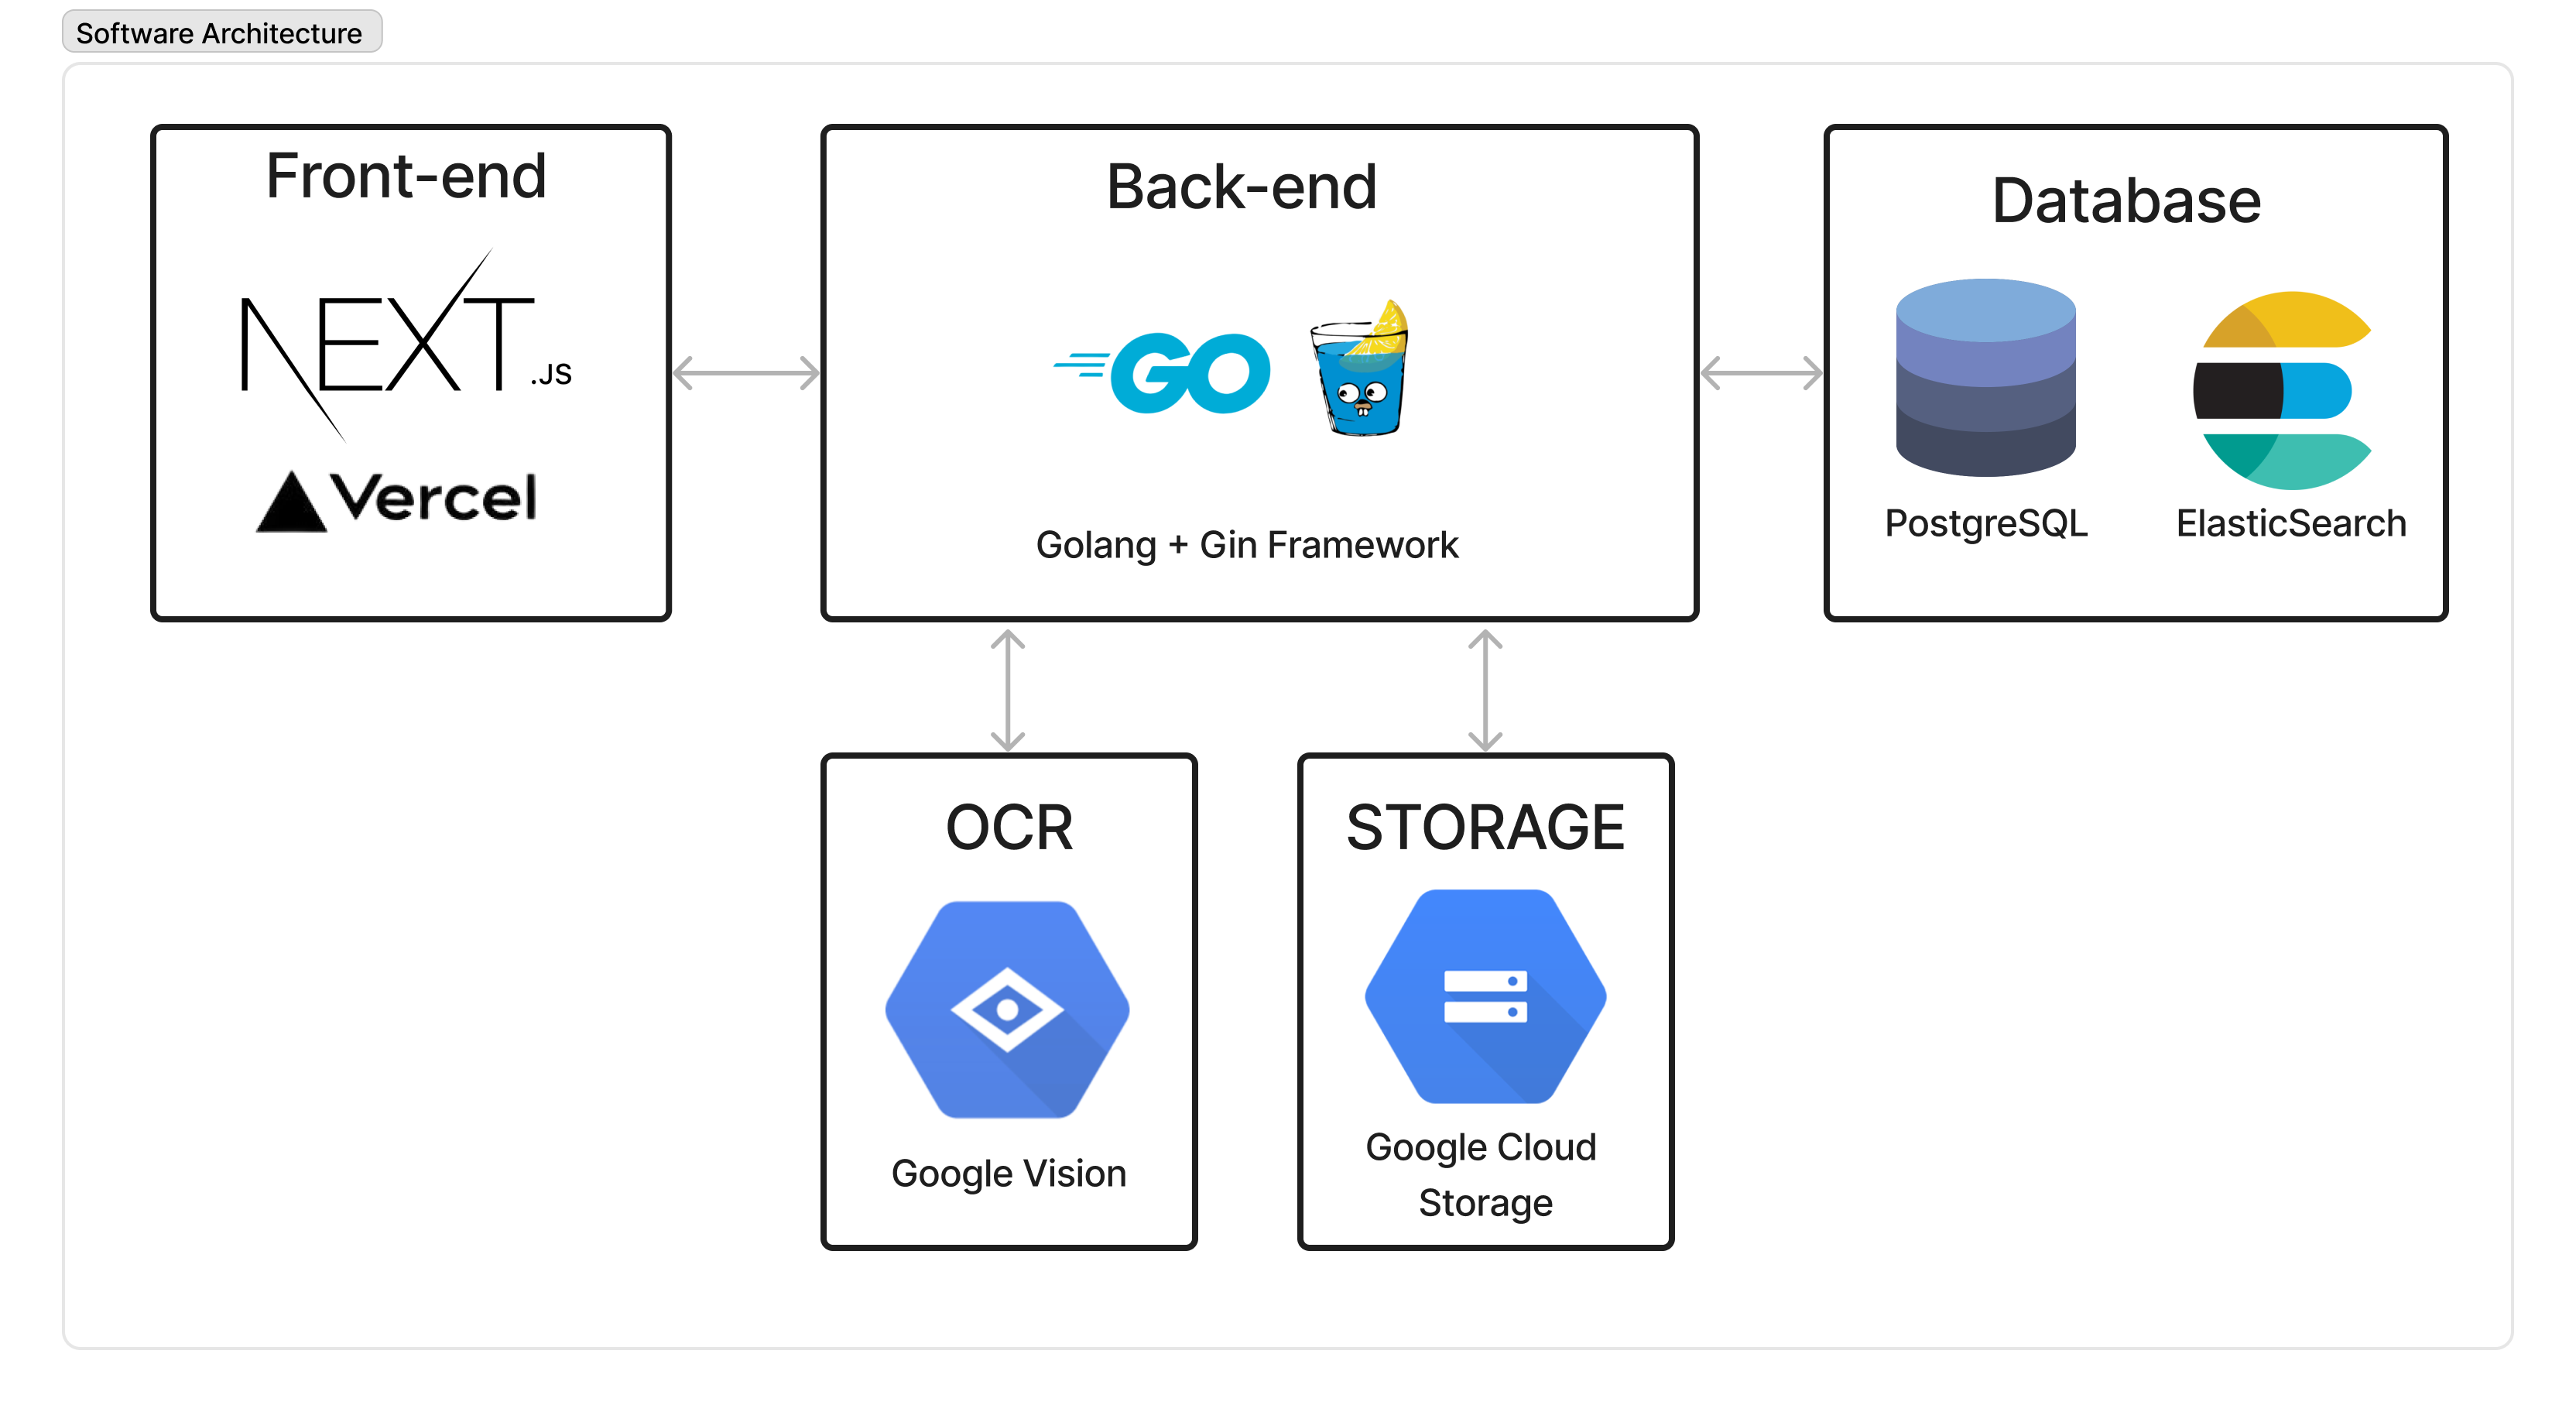
\includegraphics[width=13cm]{./assets/software-architecture.png}
  \caption{รูปแสดงสถาปัตยกรรมระบบของซอฟแวร์}\label{fig:systemArch}
\end{figure}

\newpage
\section{ข้อกำหนดและความต้องการของระบบ}
\begin{enumerate}
  \item สามารถสร้างโฟลเดอร์(เคส)ได้
  \item สามารถจัดการข้อมูลและสิทธิการเข้าถึงโฟลเดอร์ได้
  \item สามารถลบโฟลเดอร์ได้
  \item สามารถจัดเก็บโฟลเดอร์ได้
  \item สามารถเข้าไปในโฟลเดอร์
  \item สามารถอัปโหลดไฟล์หรือเอกสารเข้าไปในโฟลเดอร์ได้
  \item สามารถดาวน์โหลดไฟล์เก่าที่เคยอัปโหลดมาแล้วได้
  \item สามารถดาวน์โหลดไฟล์หรือเอกสารที่มีสิทธิเข้าถึงได้
  \item สามารถอัพเดทสถานะของคดีได้
  \item สามารถลบเอกสารได้
  \item สามารถเผยแพร่เอกสารได้
  \item สามารถสร้าง account ให้ทนายคนอื่นได้พร้อมกรอกข้อมูลจริง
  \item สามารถสร้างกําหนดการได้เพื่อส่งกําหนดการเข้าไปยัง Google calendar และ  e-mail
  \item สามารถค้นหาเอกสารได้จากชื่อไฟล์หรือคําที่อยู่ในเอกสารที่มีสิทธิเข้าถึงได้
  \item ทุกคนสามารถดูข้อมูลในรูปแบบของแผนที่หรือแผนภูมิรูปต่างๆได้
  \item ทุกคนสามารถดาวน์โหลดเอกสารที่เผยแพร่แล้วได้
  \item ทุกคนสามารถค้นหาและติดตามสถานะของคดีต่างๆได้
\end{enumerate}

\section{Navigation map}
\hspace{1cm} โดย Navigation map จะแบ่งออกเป็น 2 ส่วน คือ ส่วนของผู้ใช้งานทั่วไปแสดงดังรูป \ref{fig:navMapGuest}และส่วนของผู้ใช้งานที่เป็นทนายแสดงดังรูป \ref{fig:navMapLawyer}โดยในส่วนของผู้ใช้งานทั่วไปเมื่อเข้าใช้งานเว็บแอปพลิเคชันจะเริ่มต้นที่หน้า Landing ซึ่งในหน้านี้มีจะมีการแสดงแผนที่จำลองหรือในรูปแบบแผนภูมิซึ่งจะสามารถไปยังหน้าอื่นๆได้ 3 หน้า โดยมีหน้าแรกคือ 
หน้า Published document list ซึ่งเป็นหน้าที่สามารถค้นหาเอกสารที่ถูกเผยแพร่แล้วได้ และเมื่อกดเลือกดูไฟล์จะทำการเข้าไปยังหน้า Preview file ซึ่งจะเป็นหน้าที่แสดงไฟล์ PDF ได้ หน้าที่สองคือหน้า Case list โดยจะสามารถดูและติดตามคดีได้ และหน้าที่สามคือ หน้า Appointment list จะเป็นหน้าที่สามารถดูนัดหมายที่ได้รับการเผยแพร่ได้ \hspace{1cm}ในส่วนของทนายความจะเริ่มต้นที่หน้า Landing จากนั้นเข้ามาหน้า Login เมื่อเข้าสู่ระบบสำเร็จจะเข้ามาที่หน้า Home ซึ่งสามารถติดตามคดีต่างๆ จัดการเอกสาร รวมไปถึงการดูนัดหมายและตั้งค่าข้อมูลส่วนตัวได้
\begin{figure}[!h]\centering
    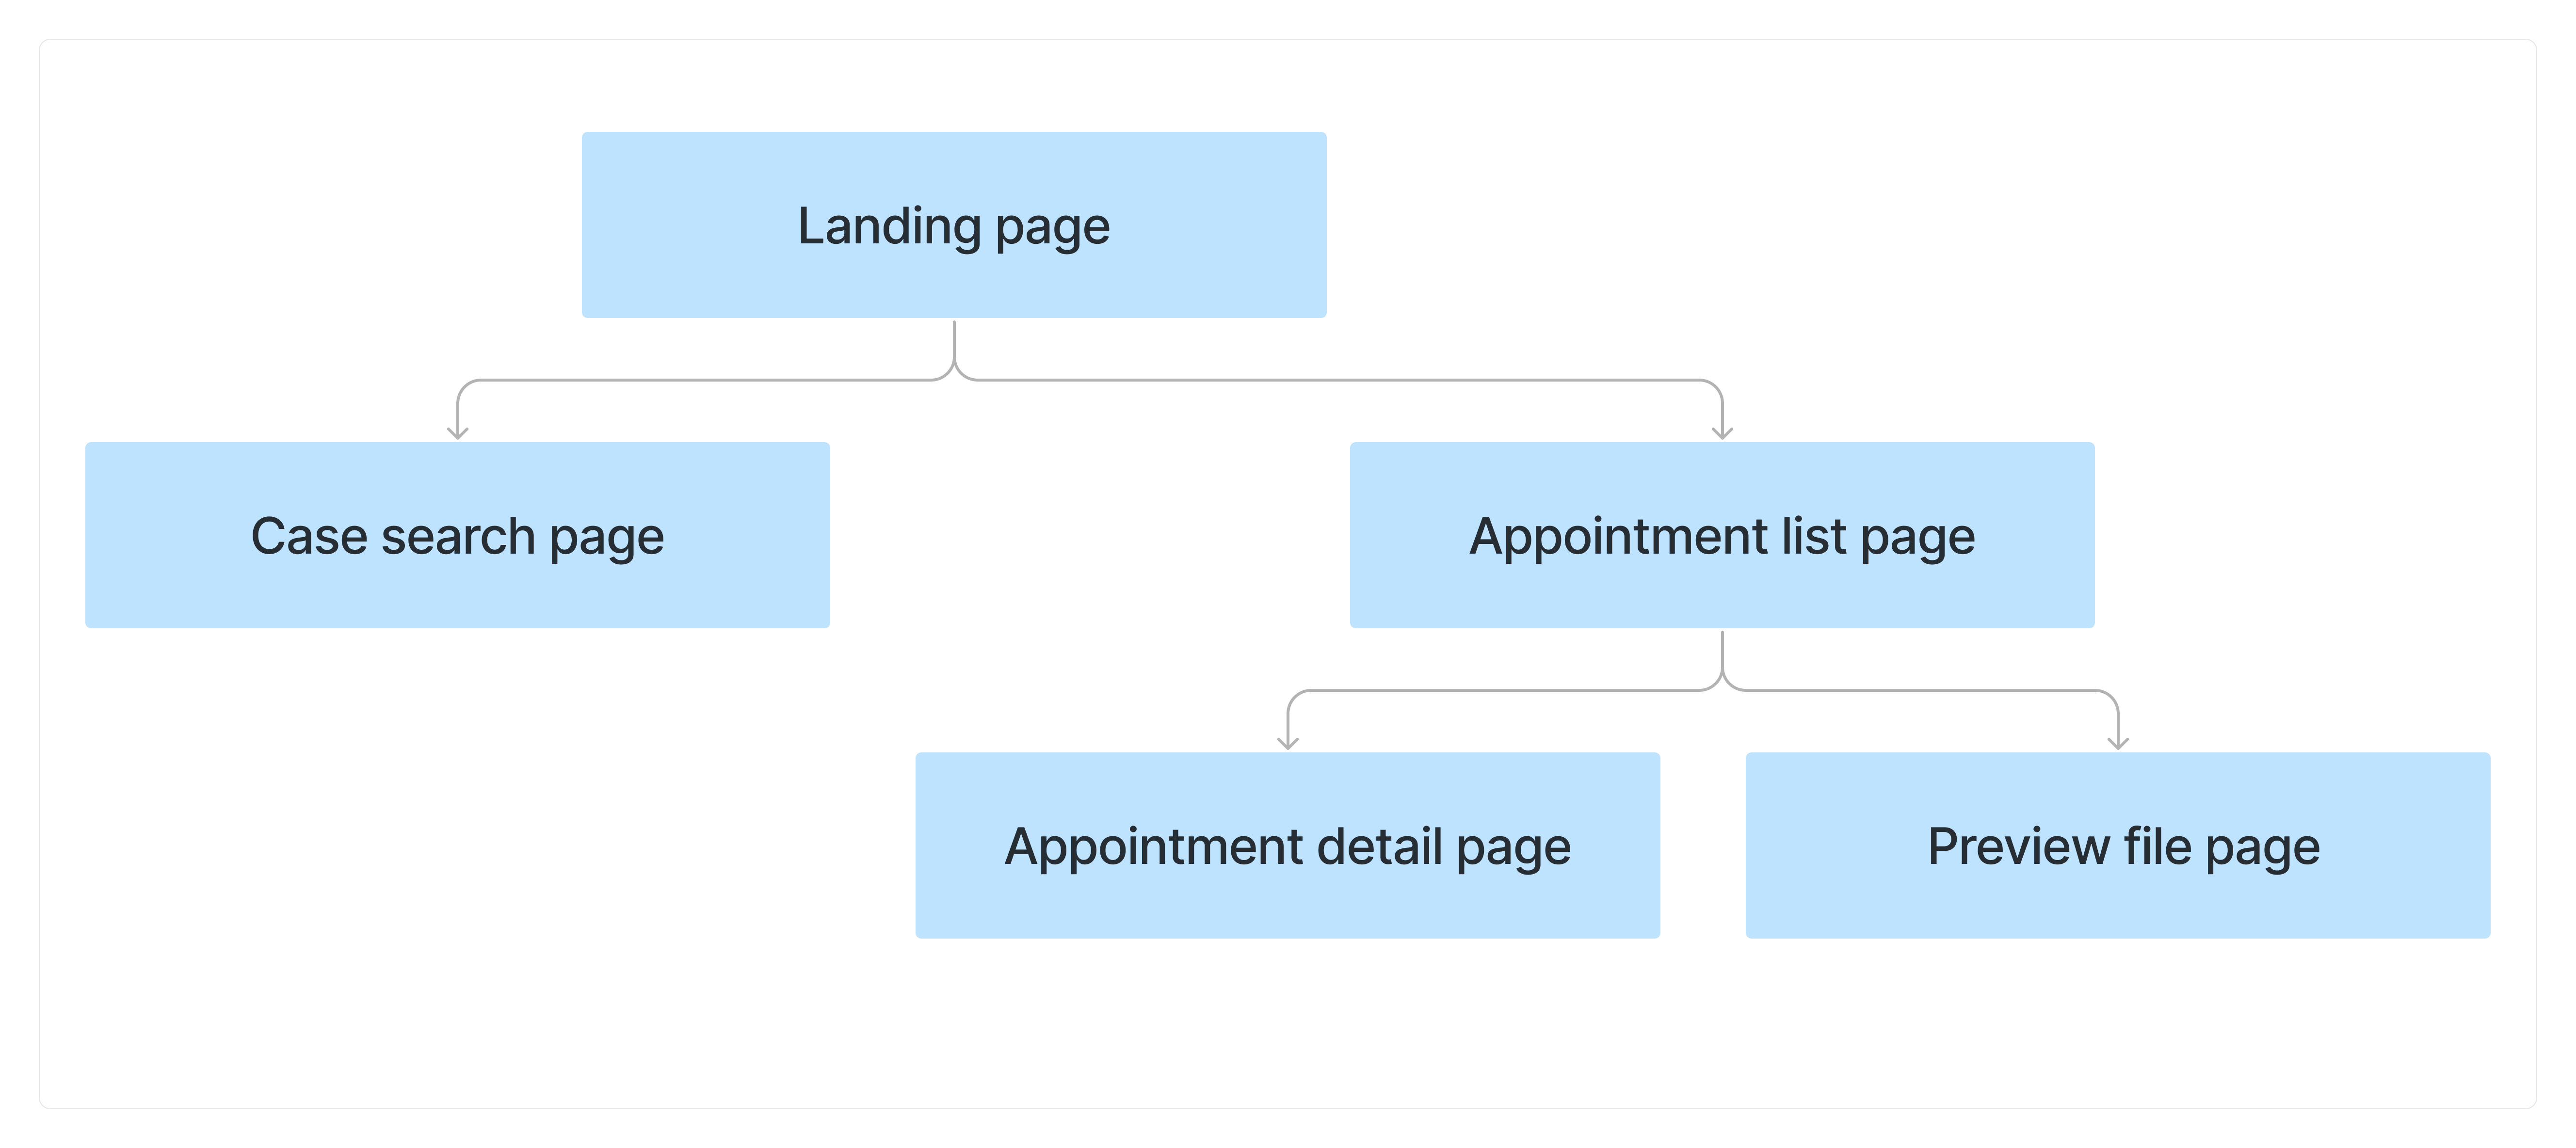
\includegraphics[width=13cm]{./assets/nav-map-guest.png}
    \caption{รูปแสดง Navigation map ของบุคคลทั่วไป}\label{fig:navMapGuest}

  \end{figure}

\begin{figure}[!h]\centering
    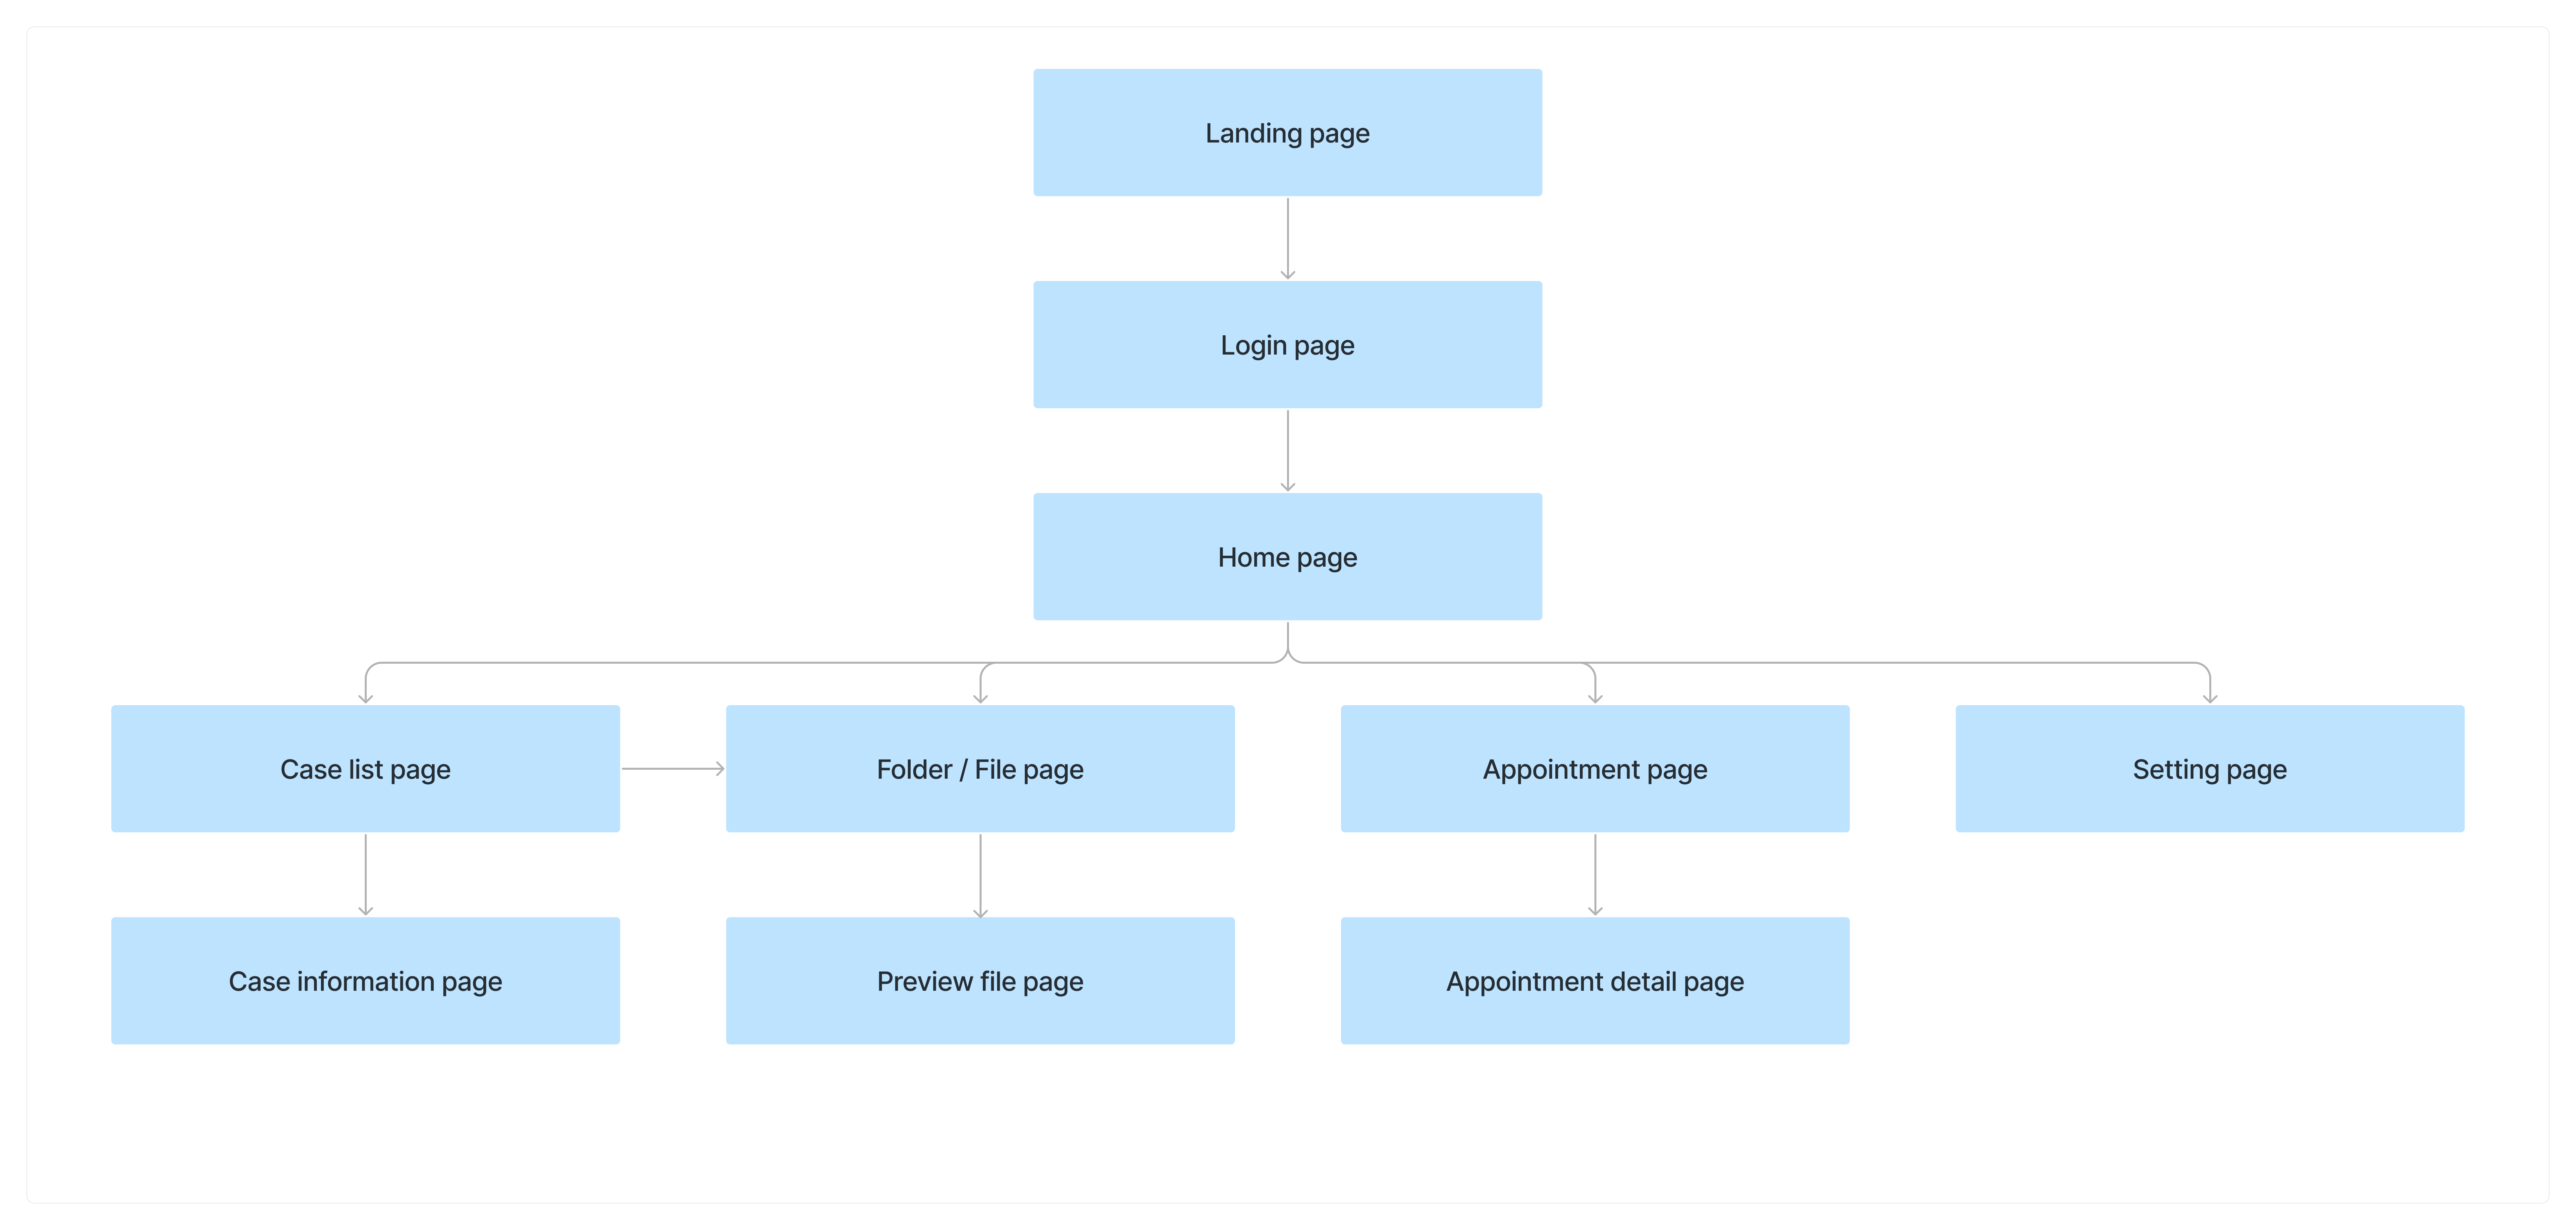
\includegraphics[width=13cm]{./assets/nav-map-lawyer.png}
    \caption{รูปแสดง Navigation map ของทนายความ}\label{fig:navMapLawyer}
\end{figure}
  

\section{โครงสร้างฐานข้อมูล}
\hspace*{1cm}โครงสร้างฐานข้อมูลของเว็บแอปพลิเคชัน DLaw แสดงดังรูป \ref{fig:erDiagram}  โดยมีรายละเอียดของชนิดตัวแปรและคํา
อธิบายเพิ่มเติมดังตารางที่ \ref{tbl:dbFileType} - \ref{tbl:dbUser} ดังนี้
\begin{figure}[!h]\centering
    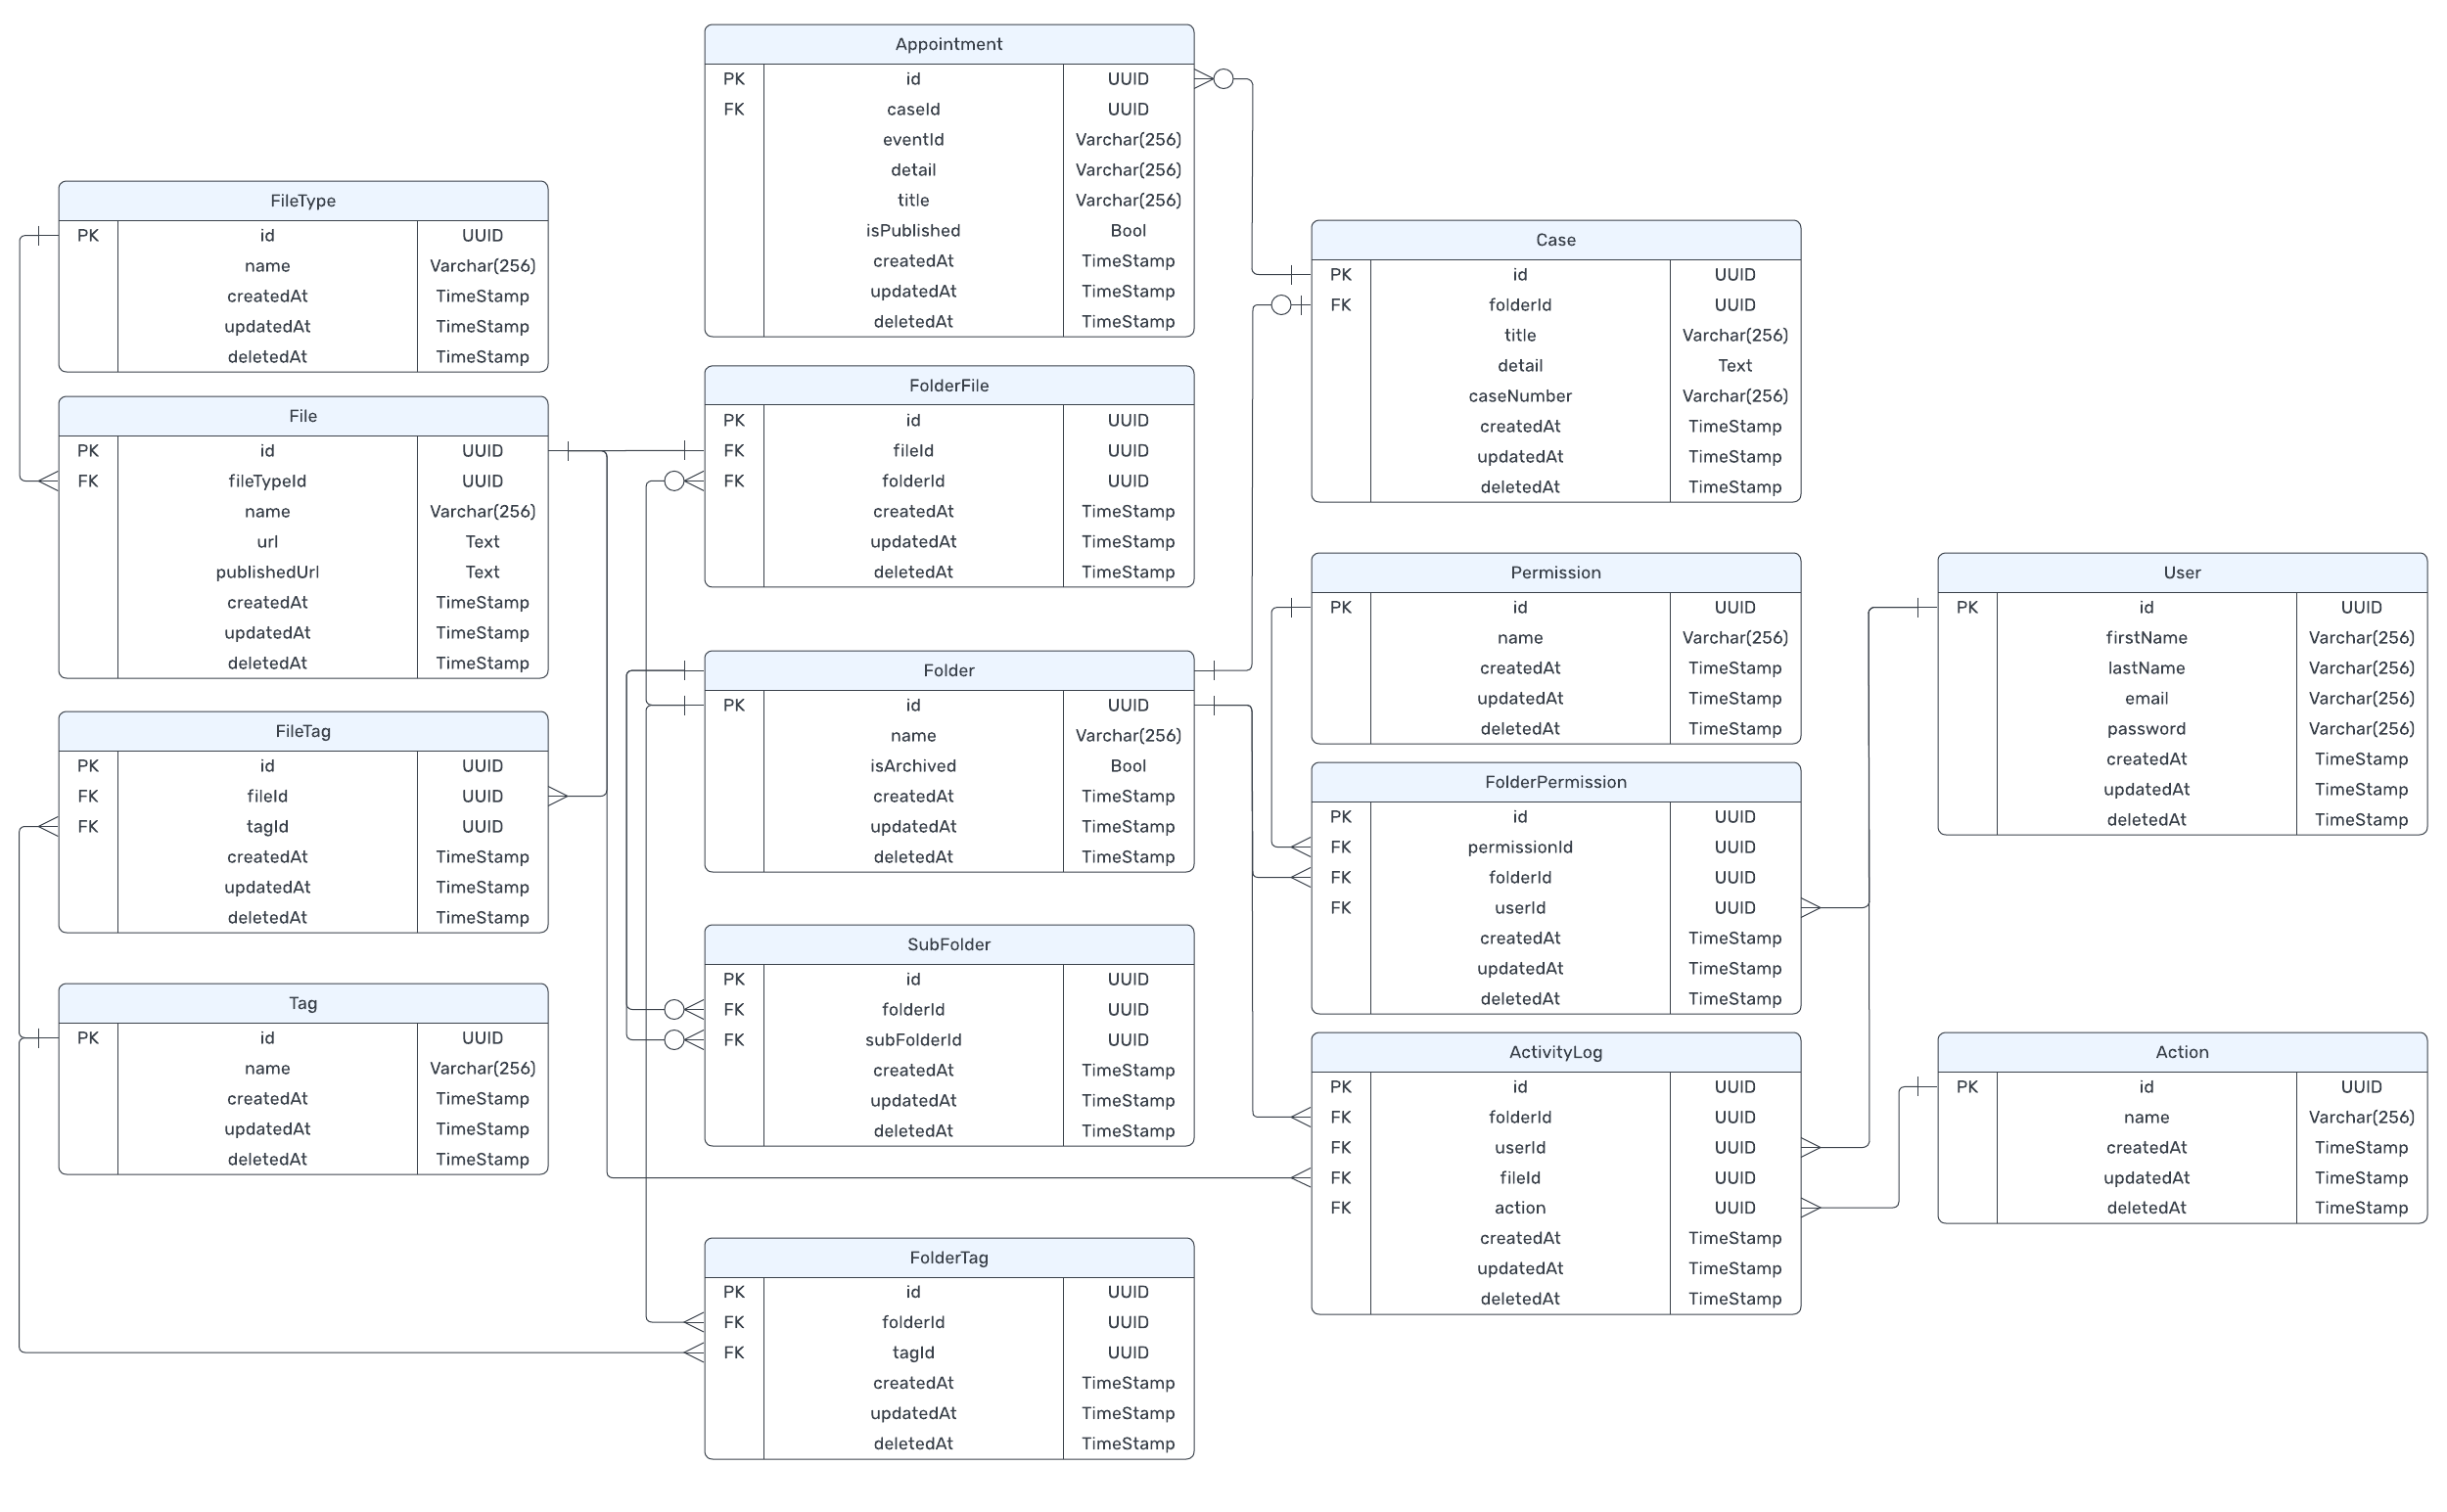
\includegraphics[width=16cm]{./assets/er-diagram.png}
    \caption{รูปแสดงโครงสร้างฐานข้อมูล}\label{fig:erDiagram}
\end{figure}

\subsection{ตาราง FileType}
ตารางที่ใช้ในการบันทึกข้อมูล ประเภทของไฟล์ในระบบ เช่น ไฟล์ประเภทเอกสาร ไฟล์ประเภทรูปภาพ เป็นต้น โดยมีรายละเอียดดังตารางที่ \ref{tbl:dbFileType}
\begin{table}[!h]
    \centering
    \begin{tabular}{|l|l|l|}
    \hline
    \textbf{Attribute} & \textbf{Type} & \textbf{Description}   \\ \hline
    id                 & UUID          & ID ของประเภทไฟล์       \\ \hline
    name               & Varchar(256)   & ชื่อของประเภทของไฟล์   \\ \hline
    createdAt          & TimeStamp     & วันเวลาที่สร้าง        \\ \hline
    updatedAt          & TimeStamp     & วันเวลาที่อัพเดทล่าสุด \\ \hline
    deletedAt          & TimeStamp     & วันเวลาที่ลบ           \\ \hline
    \end{tabular}
    \caption{\centering  ตารางแสดงรายละเอียดของตาราง FileType} \label{tbl:dbFileType}
\end{table}

\subsection{ตาราง File}
ตารางที่ใช้ในการบันทึกข้อมูลรายละเอียดไฟล์ที่ได้จากผู้ใช้งาน โดยมีรายละเอียดดังตารางที่ \ref{tbl:dbFile}
\begin{table}[!h]
    \centering
    \begin{tabular}{|l|l|l|}
    \hline
    \textbf{Attribute} & \textbf{Type} & \textbf{Description}   \\ \hline
    id                 & UUID          & ID ของไฟล์                                                      \\ \hline
    name               & Varchar(256)   & ชื่อของประเภทของไฟล์                                            \\ \hline
    fileTypeId         & UUID          & ID ของประเภทของไฟล์                                             \\ \hline
    url                & text          & Url ของไฟล์ที่ได้จาก google storage                             \\ \hline
    publishedUrl       & text          & Url ของไฟล์ที่บุคคลที่ไม่ใช่ทนายใช้ในการเข้าถึงเอกสารและดาวโหลด \\ \hline
    createdAt          & TimeStamp     & วันเวลาที่สร้าง                                                 \\ \hline
    updatedAt          & TimeStamp     & วันเวลาที่อัพเดทล่าสุด                                          \\ \hline
    deletedAt          & TimeStamp     & วันเวลาที่ลบ                                                    \\ \hline
    \end{tabular}
    \caption{\centering  ตารางแสดงรายละเอียดของตาราง File} \label{tbl:dbFile}
\end{table}

\subsection{ตาราง Tag}
ตารางที่ใช้ในการบันทึกข้อมูลรายละเอียดของแท็กต่างๆ โดยมีรายละเอียดดังตารางที่ \ref{tbl:dbTag}
\begin{table}[!h]
    \centering
    \begin{tabular}{|l|l|l|}
    \hline
    \textbf{Attribute} & \textbf{Type} & \textbf{Description}   \\ \hline
    id                 & UUID          & ID ของ tag             \\ \hline
    name               & Varchar(256)   & ชื่อ tag               \\ \hline
    createdAt          & TimeStamp     & วันเวลาที่สร้าง        \\ \hline
    updatedAt          & TimeStamp     & วันเวลาที่อัพเดทล่าสุด \\ \hline
    deletedAt          & TimeStamp     & วันเวลาที่ลบ       \\ \hline
    \end{tabular}
    \caption{\centering  ตารางแสดงรายละเอียดของตาราง Tag} \label{tbl:dbTag}
\end{table}

\subsection{ตาราง FileTag}
ตารางที่ใช้ในการบันทึกข้อมูลความสัมพันธ์ระหว่าง file กับ Tag โดยที่ว่า ใน 1 ไฟล์นั้นสามารถมีได้หลาย Tag โดยมีรายละเอียดดังตารางที่ \ref{tbl:dbFileTag}
\begin{table}[!h]
    \centering
    \begin{tabular}{|l|l|l|}
    \hline
    \textbf{Attribute} & \textbf{Type} & \textbf{Description}   \\ \hline
    id                 & UUID          & ID ของ file tag        \\ \hline
    fileId             & UUID          & ID ของ file            \\ \hline
    tagId              & UUID          & ID ของ tag             \\ \hline
    createdAt          & TimeStamp     & วันเวลาที่สร้าง        \\ \hline
    updatedAt          & TimeStamp     & วันเวลาที่อัพเดทล่าสุด \\ \hline
    deletedAt          & TimeStamp     & วันเวลาที่ลบ          \\ \hline
    \end{tabular}
    \caption{\centering  ตารางแสดงรายละเอียดของตาราง FileTag} \label{tbl:dbFileTag}
\end{table}

\subsection{ตาราง Folder}
ตารางที่ใช้ในการบันทึกข้อมูลรายละเอียดโฟลเดอร์โดยจะมี attribute ที่มีชื่อว่า isArchived มาใช้ในการบ่งบอกว่าโฟลเดอร์นี้สามารถใช้งานได้หรือไม่โดยมีรายละเอียดดังตารางที่ \ref{tbl:dbFolder}
\begin{table}[!h]
    \centering
    \begin{tabular}{|l|l|l|}
    \hline
    \textbf{Attribute} & \textbf{Type} & \textbf{Description}   \\ \hline
    id        & UUID        & ID ของ folder          \\ \hline
    name      & Varchar(256) & ชื่อ folder            \\ \hline
    isArchived         & Boolean          & เก็บถาวรหรือเป็น attribute ที่บ่งบอกถึงสถานะการใช้งานว่าใช้ได้หรือไม่ \\ \hline
    createdAt & TimeStamp   & วันเวลาที่สร้าง        \\ \hline
    updatedAt & TimeStamp   & วันเวลาที่อัพเดทล่าสุด \\ \hline
    deletedAt & TimeStamp   & วันเวลาที่ลบ             \\ \hline
    \end{tabular}
    \caption{\centering  ตารางแสดงรายละเอียดของตาราง Folder} \label{tbl:dbFolder}
\end{table}


\subsection{ตาราง FolderFile}
ตารางที่ใช้ในการบันทึกข้อมูลว่าโฟลเดอร์นั้นๆเก็บไฟล์อะไรไว้บ้าง โดยมีรายละเอียดดังตารางที่  \ref{tbl:dbFolderFile}
\begin{table}[!h]
    \centering
    \begin{tabular}{|l|l|l|}
    \hline
    \textbf{Attribute} & \textbf{Type} & \textbf{Description}   \\ \hline
    id        & UUID      & ID ของ folder file     \\ \hline
    flieId    & UUID      & ID ของ file            \\ \hline
    folderId  & UUID      & ID ของ folder          \\ \hline
    createdAt & TimeStamp & วันเวลาที่สร้าง        \\ \hline
    updatedAt & TimeStamp & วันเวลาที่อัพเดทล่าสุด \\ \hline
    deletedAt & TimeStamp & วันเวลาที่ลบ              \\ \hline
    \end{tabular}
    \caption{\centering  ตารางแสดงรายละเอียดของตาราง FolderFile} \label{tbl:dbFolderFile}
\end{table}

\subsection{ตาราง SubFolder}
ตารางที่ใช้ในการบันทึกข้อมูลรายละเอียดไฟล์โดยมีรายละเอียดดังตารางที่ \ref{tbl:dbSubFolder}
\begin{table}[!h]
    \centering
    \begin{tabular}{|l|l|l|}
    \hline
    \textbf{Attribute} & \textbf{Type} & \textbf{Description}   \\ \hline
    id          & UUID      & ID ของ record                \\ \hline
    folderId    & UUID      & ID ของโฟลเดอร์ที่อยู่ด้านนอก \\ \hline
    subFolderId & UUID      & ID ของโฟลเดอร์ที่อยู่ด้านใน  \\ \hline
    createdAt   & TimeStamp & วันเวลาที่สร้าง              \\ \hline
    updatedAt   & TimeStamp & วันเวลาที่อัพเดทล่าสุด       \\ \hline
    deletedAt   & TimeStamp & วันเวลาที่ลบ                \\ \hline  
    \end{tabular}
    \caption{\centering  ตารางแสดงรายละเอียดของตาราง SubFolder} \label{tbl:dbSubFolder}
\end{table}


\subsection{ตาราง FolderTag}
ตารางที่ใช้ในการบันทึกข้อมูลรายละเอียดไฟล์โดยมีรายละเอียดดังตารางที่ \ref{tbl:dbFolderTag}
\begin{table}[!h]
    \centering
    \begin{tabular}{|l|l|l|}
    \hline
    \textbf{Attribute} & \textbf{Type} & \textbf{Description}   \\ \hline
    id        & UUID      & ID ของ record          \\ \hline
    folderId  & UUID      & ID ของ folder          \\ \hline
    tagId     & UUID      & ID ของ tag             \\ \hline
    createdAt & TimeStamp & วันเวลาที่สร้าง        \\ \hline
    updatedAt & TimeStamp & วันเวลาที่อัพเดทล่าสุด \\ \hline
    deletedAt & TimeStamp & วันเวลาที่ลบ     \\ \hline
    \end{tabular}
    \caption{\centering  ตารางแสดงรายละเอียดของตาราง FolderTag} \label{tbl:dbFolderTag}
\end{table}



\subsection{ตาราง Case}
ตารางที่ใช้ในการบันทึกข้อมูลรายละเอียดคดีในแต่ละคดี โดยมีรายละเอียดดังตารางที่ \ref{tbl:dbCase}
\begin{table}[!h]
    \centering
    \begin{tabular}{|l|l|l|}
    \hline
    \textbf{Attribute} & \textbf{Type} & \textbf{Description}   \\ \hline
    id         & UUID        & ID ของ case                 \\ \hline
    folderId   & UUID        & ID ของ folder ที่เชื่อมอยู่ \\ \hline
    title      & Varchar(256) & ชื่อคดี                     \\ \hline
    detail     & text        & รายละเอียดคดี               \\ \hline
    caseNumber & Varchar(256) & เลขคดี                      \\ \hline
    createdAt  & TimeStamp   & วันเวลาที่สร้าง             \\ \hline
    updatedAt  & TimeStamp   & วันเวลาที่อัพเดทล่าสุด      \\ \hline
    deletedAt  & TimeStamp   & วันเวลาที่ลบ     \\ \hline
    \end{tabular}
    \caption{\centering  ตารางแสดงรายละเอียดของตาราง Case} \label{tbl:dbCase}
\end{table}


\subsection{ตาราง Appointment}
ตารางที่ใช้ในการบันทึกการนัดหมาย โดยจะมี attribute isPublished มาใช้ในการบ่งบอกว่า นัดหมายในครั้งนี้สามารถเปิดเผยสู่สาธารณะได้หรือไม่ และมี eventId ที่ได้มาจากการสร้าง event ผ่าน Google calendar api โดยมีรายละเอียดดังตารางที่  \ref{tbl:dbAppointment}
\begin{table}[!h]
    \centering
    \begin{tabular}{|l|l|l|}
    \hline
    \textbf{Attribute} & \textbf{Type} & \textbf{Description}   \\ \hline
    id          & UUID        & ID ของ appointment                        \\ \hline
    caseId      & UUID        & ID ของ case                               \\ \hline
    eventId     & Varchar(256) & ID ของ event ที่ใช้ใน google calendar api \\ \hline
    detail      & Varchar(256) & รายละเอียดของการนัดหมาย                   \\ \hline
    title       & Varchar(256) & ชื่อของการนัดหมาย                         \\ \hline
    isPublished & Boolean        & เปิดเผยสู่สาธารณะหรือไม่                  \\ \hline
    createdAt   & TimeStamp   & วันเวลาที่สร้าง                           \\ \hline
    updatedAt   & TimeStamp   & วันเวลาที่อัพเดทล่าสุด                    \\ \hline
    deletedAt   & TimeStamp   & วันเวลาที่ลบ             \\ \hline
    \end{tabular}
    \caption{\centering  ตารางแสดงรายละเอียดของตาราง Appointment} \label{tbl:dbAppointment}
\end{table}


\subsection{ตาราง Permission}
ตารางที่ใช้ในการบันทึกข้อมูลรายสิทธิในการเข้าถึงที่มีอยู่ในระบบ โดยมีรายละเอียดดังตารางที่ \ref{tbl:dbPermission}
\begin{table}[!h]
    \centering
    \begin{tabular}{|l|l|l|}
    \hline
    \textbf{Attribute} & \textbf{Type} & \textbf{Description}   \\ \hline
    id        & UUID        & ID ของ permission      \\ \hline
    name      & Varchar(256) & ชื่อของ permission     \\ \hline
    createdAt & TimeStamp   & วันเวลาที่สร้าง        \\ \hline
    updatedAt & TimeStamp   & วันเวลาที่อัพเดทล่าสุด \\ \hline
    deletedAt & TimeStamp   & วันเวลาที่ลบ                \\ \hline
    \end{tabular}
    \caption{\centering  ตารางแสดงรายละเอียดของตาราง Permission} \label{tbl:dbPermission}
\end{table}


\subsection{ตาราง FolderPermission}
ตารางที่ใช้ในการบันทึกข้อมูลรายละเอียดไฟล์ที่เชื่อมความสัมพันธ์ระหว่างสิทธิของผู้ใช้งานกับโฟลเดอร์ โดยมีรายละเอียดดังตารางที่ \ref{tbl:dbFolderPermission}
\begin{table}[!h]
    \centering
    \begin{tabular}{|l|l|l|}
    \hline
    \textbf{Attribute} & \textbf{Type} & \textbf{Description}   \\ \hline
    id           & UUID      & ID ของ folder appointment \\ \hline
    permissionId & UUID      & ID ของ permission         \\ \hline
    folderId     & UUID      & ID ของ folder             \\ \hline
    userId       & UUID      & ID ของ user               \\ \hline
    createdAt    & TimeStamp & วันเวลาที่สร้าง           \\ \hline
    updatedAt    & TimeStamp & วันเวลาที่อัพเดทล่าสุด    \\ \hline
    deletedAt    & TimeStamp & วันเวลาที่ลบ            \\ \hline
    \end{tabular}
    \caption{\centering  ตารางแสดงรายละเอียดของตาราง FolderPermission} \label{tbl:dbFolderPermission}
\end{table}


\subsection{ตาราง ActivityLog}
ตารางที่ใช้ในการบันทึกข้อมูลการอัพเดทไฟล์ที่เกิดขึ้นในแต่ละโฟลเดอร์ โดยมีรายละเอียดดังตารางที่ \ref{tbl:dbActivityLog}
\begin{table}[!h]
    \centering
    \begin{tabular}{|l|l|l|}
    \hline
    \textbf{Attribute} & \textbf{Type} & \textbf{Description}   \\ \hline
    id        & UUID      & ID ของ activity log                 \\ \hline
    folderId  & UUID      & ID ของ folder ที่ถูกทำการอัพเดทไฟล์ \\ \hline
    userId    & UUID      & ID ของ user ที่ทำการอัพเดทไฟล์      \\ \hline
    flieId    & UUID      & ID ของ file ที่ถูกทำการอัพเดท       \\ \hline
    actionId  & UUID      & ID ของ action ที่ทำ                 \\ \hline
    createdAt & TimeStamp & วันเวลาที่สร้าง                     \\ \hline
    updatedAt & TimeStamp & วันเวลาที่อัพเดทล่าสุด              \\ \hline
    deletedAt & TimeStamp & วันเวลาที่ลบ                      \\ \hline
    \end{tabular}
    \caption{\centering  ตารางแสดงรายละเอียดของตาราง ActivityLog} \label{tbl:dbActivityLog}
\end{table}


\subsection{ตาราง Action}
ตารางที่ใช้ในการบันทึกข้อมูลรายละเอียดของการทำ activity เช่น สร้าง อัพเดท ลบ โดยมีรายละเอียดดังตารางที่ \ref{tbl:dbAction}
\begin{table}[!h]
    \centering
    \begin{tabular}{|l|l|l|}
    \hline
    \textbf{Attribute} & \textbf{Type} & \textbf{Description}   \\ \hline
    id        & UUID        & ID ของ action          \\ \hline
    name      & Varchar(256) & ชื่อของ action         \\ \hline
    createdAt & TimeStamp   & วันเวลาที่สร้าง        \\ \hline
    updatedAt & TimeStamp   & วันเวลาที่อัพเดทล่าสุด \\ \hline
    deletedAt & TimeStamp   & วันเวลาที่ลบ          \\ \hline    
    \end{tabular}
    \caption{\centering  ตารางแสดงรายละเอียดของตาราง Action} \label{tbl:dbAction}
\end{table}


\subsection{ตาราง User}
ตารางที่ใช้ในการบันทึกข้อมูลรายละเอียดผู้ใช้งาน โดยมีรายละเอียดดังตารางที่ \ref{tbl:dbUser}
\begin{table}[!h]
    \centering
    \begin{tabular}{|l|l|l|}
    \hline
    \textbf{Attribute} & \textbf{Type} & \textbf{Description}   \\ \hline
    id        & UUID        & ID ของ user            \\ \hline
    firstName & Varchar(256) & ชื่อจริง               \\ \hline
    lastName  & Varchar(256) & นามสกุล                \\ \hline
    email     & Varchar(256) & อีเมล์                 \\ \hline
    password  & Varchar(256) & รหัสผ่าน               \\ \hline
    createdAt & TimeStamp   & วันเวลาที่สร้าง        \\ \hline
    updatedAt & TimeStamp   & วันเวลาที่อัพเดทล่าสุด \\ \hline
    deletedAt & TimeStamp   & วันเวลาที่ลบ                \\ \hline
    \end{tabular}
    \caption{\centering  ตารางแสดงรายละเอียดของตาราง User} \label{tbl:dbUser}
\end{table}


\section{Use case diagram}


\section{Use case narrative}




%%%%%%%%%%%%%%%%%%%%%%%%%%%%%%%%%%%%%%%%%%%%%%%%%%%%%%%%%%%%
%%%%%%%%%%%%%%%%%%%%%%% CHAPTER4 %%%%%%%%%%%%%%%%%%%%%%%%%%%
%%%%%%%%%%%%%%%%%%%%%%%%%%%%%%%%%%%%%%%%%%%%%%%%%%%%%%%%%%%%
\chapter{ผลการดำเนินงาน}

You can title this chapter as \textbf{Preliminary Results} ผลการดำเนินงานเบื้องต้น or \textbf{Work Progress} ความก้าวหน้าโครงงาน for the progress reports. Present implementation or experimental results here and discuss them.
ใส่เฉพาะหัวข้อที่เกี่ยวข้องกับงานที่ทำ 

\section{ประสิทฺธิภาพการทำงานของระบบ} 
\section{ความพึงพอใจการใช้งาน}
\section{การวิเคราะห์ข้อมูลและผลการทดลอง}

%%%%%%%%%%%%%%%%%%%%%%%%%%%%%%%%%%%%%%%%%%%%%%%%%%%%%%%%%%%%
%%%%%%%%%%%%%%%%%%%%%%% CHAPTER5 %%%%%%%%%%%%%%%%%%%%%%%%%%%
%%%%%%%%%%%%%%%%%%%%%%%%%%%%%%%%%%%%%%%%%%%%%%%%%%%%%%%%%%%%
\chapter{บทสรุป}

This chapter is optional for proposal and progress reports but 
is required for the final report.

\section{สรุปผลโครงงาน}
สรุปว่าโครงงานบรรลุตามวัตถุประสงค์ที่ตั้งไว้หรือไม่ อย่างไร 

\section{ปัญหาที่พบและการแก้ไข}
State your problems and how you fixed them.

\section{ข้อจำกัดและข้อเสนอแนะ}
ข้อจำกัดของโครงงาน What could be done in the future to make your projects better.

%%%%%%%%%%%%%%%%%%%%%%%%%%%%%%%%%%%%%%%%%%%%%%%%%%%%%%%%%%%%%%%
%%%%%%%%%%%%%%%%%%%% Bibliography %%%%%%%%%%%%%%%%%%%%%%%%%%%%%
%%%%%%%%%%%%%%%%%%%%%%%%%%%%%%%%%%%%%%%%%%%%%%%%%%%%%%%%%%%%%%%

%%%% Comment this in your report to show only references you have
%%%% cited. Otherwise, all the references below will be shown.
%\nocite{*}
%% Use the kmutt.bst for bibtex bibliography style 
%% You must have cpe.bib and string.bib in your current directory.
%% You may go to file .bbl to manually edit the bib items.

\makeatletter
\g@addto@macro{\UrlBreaks}{\UrlOrds}
\makeatother

\bibliographystyle{kmutt}
\bibliography{string,cpe}

%%%%%%%%%%%%%%%%%%%%%%%%%%%%%%%%%%%%%%%%%%%%%%%%%%%%%%%%%%%%%%%
%%%%%%%%%%%%%%%%%%%%%%%% Appendix %%%%%%%%%%%%%%%%%%%%%%%%%%%%%
%%%%%%%%%%%%%%%%%%%%%%%%%%%%%%%%%%%%%%%%%%%%%%%%%%%%%%%%%%%%%%%
\appendix{ชื่อภาคผนวกที่ 1}
\noindent{\large\bf ใส่หัวข้อตามความเหมาะสม} \\





\end{document}
